\documentclass[11pt,]{article}
\usepackage[left=1in,top=1in,right=1in,bottom=1in]{geometry}
\newcommand*{\authorfont}{\fontfamily{phv}\selectfont}
\usepackage[]{mathpazo}


  \usepackage[T1]{fontenc}
  \usepackage[utf8]{inputenc}



\usepackage{abstract}
\renewcommand{\abstractname}{}    % clear the title
\renewcommand{\absnamepos}{empty} % originally center

\renewenvironment{abstract}
 {{%
    \setlength{\leftmargin}{0mm}
    \setlength{\rightmargin}{\leftmargin}%
  }%
  \relax}
 {\endlist}

\makeatletter
\def\@maketitle{%
  \newpage
%  \null
%  \vskip 2em%
%  \begin{center}%
  \let \footnote \thanks
    {\fontsize{18}{20}\selectfont\raggedright  \setlength{\parindent}{0pt} \@title \par}%
}
%\fi
\makeatother




\setcounter{secnumdepth}{3}

\usepackage{color}
\usepackage{fancyvrb}
\newcommand{\VerbBar}{|}
\newcommand{\VERB}{\Verb[commandchars=\\\{\}]}
\DefineVerbatimEnvironment{Highlighting}{Verbatim}{commandchars=\\\{\}}
% Add ',fontsize=\small' for more characters per line
\usepackage{framed}
\definecolor{shadecolor}{RGB}{248,248,248}
\newenvironment{Shaded}{\begin{snugshade}}{\end{snugshade}}
\newcommand{\KeywordTok}[1]{\textcolor[rgb]{0.13,0.29,0.53}{\textbf{#1}}}
\newcommand{\DataTypeTok}[1]{\textcolor[rgb]{0.13,0.29,0.53}{#1}}
\newcommand{\DecValTok}[1]{\textcolor[rgb]{0.00,0.00,0.81}{#1}}
\newcommand{\BaseNTok}[1]{\textcolor[rgb]{0.00,0.00,0.81}{#1}}
\newcommand{\FloatTok}[1]{\textcolor[rgb]{0.00,0.00,0.81}{#1}}
\newcommand{\ConstantTok}[1]{\textcolor[rgb]{0.00,0.00,0.00}{#1}}
\newcommand{\CharTok}[1]{\textcolor[rgb]{0.31,0.60,0.02}{#1}}
\newcommand{\SpecialCharTok}[1]{\textcolor[rgb]{0.00,0.00,0.00}{#1}}
\newcommand{\StringTok}[1]{\textcolor[rgb]{0.31,0.60,0.02}{#1}}
\newcommand{\VerbatimStringTok}[1]{\textcolor[rgb]{0.31,0.60,0.02}{#1}}
\newcommand{\SpecialStringTok}[1]{\textcolor[rgb]{0.31,0.60,0.02}{#1}}
\newcommand{\ImportTok}[1]{#1}
\newcommand{\CommentTok}[1]{\textcolor[rgb]{0.56,0.35,0.01}{\textit{#1}}}
\newcommand{\DocumentationTok}[1]{\textcolor[rgb]{0.56,0.35,0.01}{\textbf{\textit{#1}}}}
\newcommand{\AnnotationTok}[1]{\textcolor[rgb]{0.56,0.35,0.01}{\textbf{\textit{#1}}}}
\newcommand{\CommentVarTok}[1]{\textcolor[rgb]{0.56,0.35,0.01}{\textbf{\textit{#1}}}}
\newcommand{\OtherTok}[1]{\textcolor[rgb]{0.56,0.35,0.01}{#1}}
\newcommand{\FunctionTok}[1]{\textcolor[rgb]{0.00,0.00,0.00}{#1}}
\newcommand{\VariableTok}[1]{\textcolor[rgb]{0.00,0.00,0.00}{#1}}
\newcommand{\ControlFlowTok}[1]{\textcolor[rgb]{0.13,0.29,0.53}{\textbf{#1}}}
\newcommand{\OperatorTok}[1]{\textcolor[rgb]{0.81,0.36,0.00}{\textbf{#1}}}
\newcommand{\BuiltInTok}[1]{#1}
\newcommand{\ExtensionTok}[1]{#1}
\newcommand{\PreprocessorTok}[1]{\textcolor[rgb]{0.56,0.35,0.01}{\textit{#1}}}
\newcommand{\AttributeTok}[1]{\textcolor[rgb]{0.77,0.63,0.00}{#1}}
\newcommand{\RegionMarkerTok}[1]{#1}
\newcommand{\InformationTok}[1]{\textcolor[rgb]{0.56,0.35,0.01}{\textbf{\textit{#1}}}}
\newcommand{\WarningTok}[1]{\textcolor[rgb]{0.56,0.35,0.01}{\textbf{\textit{#1}}}}
\newcommand{\AlertTok}[1]{\textcolor[rgb]{0.94,0.16,0.16}{#1}}
\newcommand{\ErrorTok}[1]{\textcolor[rgb]{0.64,0.00,0.00}{\textbf{#1}}}
\newcommand{\NormalTok}[1]{#1}

\usepackage{graphicx,grffile}
\makeatletter
\def\maxwidth{\ifdim\Gin@nat@width>\linewidth\linewidth\else\Gin@nat@width\fi}
\def\maxheight{\ifdim\Gin@nat@height>\textheight\textheight\else\Gin@nat@height\fi}
\makeatother
% Scale images if necessary, so that they will not overflow the page
% margins by default, and it is still possible to overwrite the defaults
% using explicit options in \includegraphics[width, height, ...]{}
\setkeys{Gin}{width=\maxwidth,height=\maxheight,keepaspectratio}

\title{Búsqueda de Hotspots y Modelización del Analfabetismo en República
Dominicana; Geo estadística de la precipitación del 2008  }



\author{\Large Estebania de la Cruz del Rosario\vspace{0.05in} \newline\normalsize\emph{Maestrante, Universidad Autónoma de Santo Domingo (UASD)}  }


\date{}

\usepackage{titlesec}

\titleformat*{\section}{\normalsize\bfseries}
\titleformat*{\subsection}{\normalsize\itshape}
\titleformat*{\subsubsection}{\normalsize\itshape}
\titleformat*{\paragraph}{\normalsize\itshape}
\titleformat*{\subparagraph}{\normalsize\itshape}

\titlespacing{\section}
{0pt}{36pt}{0pt}
\titlespacing{\subsection}
{0pt}{36pt}{0pt}
\titlespacing{\subsubsection}
{0pt}{36pt}{0pt}





\newtheorem{hypothesis}{Hypothesis}
\usepackage{setspace}

\makeatletter
\@ifpackageloaded{hyperref}{}{%
\ifxetex
  \PassOptionsToPackage{hyphens}{url}\usepackage[setpagesize=false, % page size defined by xetex
              unicode=false, % unicode breaks when used with xetex
              xetex]{hyperref}
\else
  \PassOptionsToPackage{hyphens}{url}\usepackage[unicode=true]{hyperref}
\fi
}

\@ifpackageloaded{color}{
    \PassOptionsToPackage{usenames,dvipsnames}{color}
}{%
    \usepackage[usenames,dvipsnames]{color}
}
\makeatother
\hypersetup{breaklinks=true,
            bookmarks=true,
            pdfauthor={Estebania de la Cruz del Rosario (Maestrante, Universidad Autónoma de Santo Domingo (UASD))},
             pdfkeywords = {Analfabestimo, Precipitación, Modelizacion Espacial},  
            pdftitle={Búsqueda de Hotspots y Modelización del Analfabetismo en República
Dominicana; Geo estadística de la precipitación del 2008},
            colorlinks=true,
            citecolor=blue,
            urlcolor=blue,
            linkcolor=magenta,
            pdfborder={0 0 0}}
\urlstyle{same}  % don't use monospace font for urls

% set default figure placement to htbp
\makeatletter
\def\fps@figure{htbp}
\makeatother

\usepackage{pdflscape} \newcommand{\blandscape}{\begin{landscape}}
\newcommand{\elandscape}{\end{landscape}}


% add tightlist ----------
\providecommand{\tightlist}{%
\setlength{\itemsep}{0pt}\setlength{\parskip}{0pt}}

\begin{document}
	
% \pagenumbering{arabic}% resets `page` counter to 1 
%
% \maketitle

{% \usefont{T1}{pnc}{m}{n}
\setlength{\parindent}{0pt}
\thispagestyle{plain}
{\fontsize{18}{20}\selectfont\raggedright 
\maketitle  % title \par  

}

{
   \vskip 13.5pt\relax \normalsize\fontsize{11}{12} 
\textbf{\authorfont Estebania de la Cruz del Rosario} \hskip 15pt \emph{\small Maestrante, Universidad Autónoma de Santo Domingo (UASD)}   

}

}








\begin{abstract}

    \hbox{\vrule height .2pt width 39.14pc}

    \vskip 8.5pt % \small 

\noindent En resumen, en esta investigación donde la pregunta de Educación: ``Sabe
leer y escribir; no sabe leer ni escribir'' en cuanto a la
autocorrelación según la comprobación de homocedasticidad, para la
variable respecto de la coordenada Y, tanto grafico como la prueba de
homocedasticidad, el resultado obtenido sugiere heterocedasticidad; pero
respecto de X hay homocedasticidad. Y para el diagrama de moran plot San
Rafael del Yuma tiene mucha más población que ``no sabe leer ni
escribir'', que lo que se esperaría de acuerdo a su entorno, eso se
considera un outlayer espacial o un aberración espacial, El Mapa LISA
Cliusters, nos muestra cuales son los grumos o aglomerados del valor
alto de la variable, el valor alto de la variable es el porcentaje de
persona que ``no sabe leer ni escribir'', esa variable se comporta de la
manera grumosa en 24 municipio, En 23 municipios pasa el efecto
contrario estos municipios están autorrelacionado entre sí pero con bajo
valor de la variable, Existen Dos grumos de bajo valor de las variables
y tres grumos de alto valor de las variables. En el recto como no se
parece entre sí, no hay una autocorrelacion espacial entre ellos, no hay
una auotcorrelacion significativa. Duvergé es un caso contrario, se
esperaría un analfabetismo grande, pero se obtuvo un valor menor. Para
el proceso de la Modelización el modelo con variable cuyo coeficientes
resultaron significativo, la variable del porcentaje de persona que no
sabe leer ni escribir, están asociadas con las variables: Edad en grupos
quinquenales 0, 1-4,\ldots{}. 85 y más: 60 - 64 y Tipo de vivienda:
Barracón estos son directo y el Asiste o asistió a la escuela: No
asiste, pero asistió e inverso porque el coeficiente es negativo. Para
la Geoestadística de la Precipitación del año 2008, obtuvimos para
representar el objeto stars, según el mapa las provincias donde se
evidencian que hubo mayores precipitaciones son: Sánchez Ramírez, Monte
Plata, María Trinidad Sánchez, Santo Domingo, Distrito Nacional San José
de Ocoa, Hermanas Mirabal, San Cristóbal, Duarte, Semana, Barahona y
Monseñor Noel.


\vskip 8.5pt \noindent \emph{Keywords}: Analfabestimo, Precipitación, Modelizacion Espacial \par

    \hbox{\vrule height .2pt width 39.14pc}



\end{abstract}


\vskip 6.5pt


\noindent  \section{Introducción}\label{introducciuxf3n}

La siguiente investigación de análisis espacial se realizara con el fin
de dar a conocer la cantidad, estado, condiciones y ubicación, del
analfabetismo en República Dominicana; además obtendremos los datos e
informaciones, para esto vamos a trabajar con la pregunta ``Sabe leer y
escribir; No sabe leer ni escribir'' según (Ureña \& Martínez, n.d.) del
(ONE, 2012), todo el trabajo se vas hacer en el programa de RStudio. R
es un software gratuito que está constituido por herramientas, se pueden
ampliar por paquetes, librerías y define funciones, R es un código
abierto que nos permite ahorrar económicamente ya que es un software
libre, no es pirateado, esto es según QUÉ ES R .Nuestra finalidad en
esta investigación del analfabetismo es aplicar las múltiples
formulaciones y medidas de Autocorrelación espacial e indicar cómo el
concepto ayuda a determinar la naturaleza espacial de los datos
georreferenciados, vamos a trabajar con código, además de cargar
paquete, todo esto paquete deben estar cargado en R estudio, segun
(Bivand, Pebesma, Gomez-Rubio, \& Pebesma, 2008). La Modelización de
Datos Espaciales, es una asociación, aquí vamos a cargar una serie de
librería como son: library(tidyverse), library(sf), library(spdep) y la
library(lmtest, libreriay variableusan (Tomislav Hengl, 2009). Además
vamos a trabajar con Geoestadistica de la precipitación del año 2008,
segun (ONAMET, 2008). La Geoestadistica estudia fenómenos con relación
espacial, aquí vamos a estudiar algunos de los diferentes variogramas y
cuál será el usado para nuestra investigación, sabiendo que los
variogramas sirven para pronosticar la interpolación espacial. (Hengl,
2009).

\section{Metodología}\label{metodologuxeda}

La presente investigación busca conocer el analfabetismo de la diferente
provincia según (ONE, 2012) se hizo la siguiente pregunta ``Sabe leer y
escribir: No sabe leer ni escribir'' es muy importantes, aquí
utilizaremos el método de observación para reconocer y apreciar el
desarrollo del fenómeno que es objeto de estudio, es decir, nuestro
problema de investigación. Vamos a cargar paquetes o librerías
necesarias para que R estudio pueda obtener los datos y así tener mejor
resultados, para esto aplicaremos tres técnicas: Los Hotspots,
Asociación y Superficies Continuas. Los Hotspots, es la Autocorrelacion
Lisa Clirters (Moran), para evaluar autocorrelación se requiere conocer
tanto los datos como los supuestos. En la Asociación está la
Modelización de datos espaciales, las modelizaciones autorregresivas
requieren considerar la autocorrelación espacial, puesto que,
normalmente, las geometrías poligonales contienen observaciones que no
son independientes entre sí, con lo cual se viola uno de los supuestos
más importantes de la regresión. Las Superficies Continuas no son más
que los Datos Puntuales, Geoestadistica, Variogramas y Krigng, La
geoestadística se ocupa en modelar, predecir y simular fenómenos
espacialmente continuos; la Geoestadistica asiste en la predicción
espacialmente continua del valor de una variable. Existen varias
modalidades de krigeaje según los distintos supuestos (todas asumen que
la variación espacial es modelizable mediante el variograma). El
variograma es el gráfico de representación de estimaciones de la
semivarianza, además R dispone de los modelos comunes de variograma. En
esta Asociación de Modelización, las modelizaciones autorregresivas
requieren considerar la autocorrelación espacial, puesto que,
normalmente, las geometrías poligonales contienen observaciones que no
son independientes entre sí, con lo cual se viola uno de los supuestos
más importantes de la regresión tradicional.(Hengl, 2009)

\ldots

\section{Resultados}\label{resultados}

\subsection{Autocorrelacion Espacial}\label{autocorrelacion-espacial}

\subsubsection{Vecinos}\label{vecinos}

En el análisis de vecinos más cercanos, JUAN DE HERRERA tiene un solo
vecino y el que más tiene es la VEGA con 14 vecinos.

\subsubsection{Analisis Exploratorio de
Datos}\label{analisis-exploratorio-de-datos}

Segun el anilis exploratorio de los datos podemos ver en el mapa de la
variable original que hay 54 municipios con aproximadamente 15\% de
personas que no saben leer ni escribir, 42 con un aproximado de 20\% de
personas que no sabe leer ni escribir, 34 municipios con un aproximado
de 24\% de personas que no sabe leer ni escribir, 20 municipios de
aproximadamente 29\% de personas que no sabe leer ni escribir y 6 de los
municipios tiene un 37\% con un alto porcentaje que no sabe leer ni
escribir.

En el análisis exploratorio de los datos podemos ver en el mapa de la
variable logarítmica que hay 24 municipios con aproximadamente 3\% de
personas que no saben leer ni escribir, 51 municipios con un aproximado
de 3\% de personas que no sabe leer ni escribir, 48 municipios con un
aproximado de 3\% de personas que no sabe leer ni escribir, 27
municipios con aproximadamente 3\% de las personas no sabe leer ni
escribir y 5 municipios de aproximadamente 4\% de las personas no sabe
leer ni escribir.

\subsubsection{Diagrama Cuantilar
Normal}\label{diagrama-cuantilar-normal}

Según el diagrama cuantilar normal, la gráfica logarítmica presenta más
normalidad en los datos, ya que se asemeja más a una línea reta.

\subsubsection{Prueba de Shapiro-Wilk}\label{prueba-de-shapiro-wilk}

Para la prueba de Shapiro-Wilk al menos los datos transformados, sí
cumplen en principio, con el supuesto de normalidad.

\subsubsection{Comprobacion de
Homocedasticidad}\label{comprobacion-de-homocedasticidad}

Según la comprobación de homocedasticidad, para la variable respecto de
la coordenada Y, tanto grafico como la prueba de homocedasticidad, el
resultado obtenido sugiere heterocedasticidad. Pero respecto de X hay
homocedasticidad.

\subsubsection{Evaluar la Autocorrelacion Espacial
Global}\label{evaluar-la-autocorrelacion-espacial-global}

En esta investigación se rechaza la hipótesis nula, porque el
coeficiente de significancia es menor que 0.05.

\subsubsection{Prueba de I Moran Local}\label{prueba-de-i-moran-local}

En el diagrama de Moran Plot San Rafael del Yuma, tiene un valor de la
variable en el eje X de 3.2, en el eje Y de acuerdo a su vecindad se
esperaría de 2.8, San Rafael del Yuma tiene mucha más población que no
sabe leer ni escribir, que lo que se esperaría de acuerdo a su entorno,
eso se considera un outlayer espacial o un aberración espacial. En San
Rafael del Yuma se observó un valor grande, pero se espera un valor más
pequeño. Duvergé es un caso contrario, se obtiene un valor de la
variable de 2.9, pero de acuerdo a su vecindad, Duvergé se esperaría es
3.4, se esperaría un analfabetismo grande, pero se obtuvo un valor
menor.

\subsubsection{Generacion de Mapa LISA}\label{generacion-de-mapa-lisa}

El Mapa LISA Cliusters, nos muestra cuales son los grumos o aglomerados
del valor alto de la variable, el valor alto de la variable es el
porcentaje de persona que no sabe leer ni escribir, esa variable se
comporta de la manera grumosa en 24 municipio, entre estos están: la
región Enriquillo en una parte de ella y en esos municipio y en algunos
municipios de la región fronteriza y también al norte de la provincia de
Azua, eso son los aglomerados donde los municipios de ese grumo se
parecen a su entorno en cuanto a esa variable, es decir Pedernales se
parece a Oviedo, Oviedo se parece a Paraíso, entre sí en cuanto al valor
de la variable, es decir están autocorrelacionado espacialmente en
cuanto a esa variable. En 23 municipios pasa el efecto contrario estos
municipios están autorrelacionado entre sí pero con bajo valor de la
variable, la variable tiene un bajo valor en Santo Domingo, San
Cristóbal, Santo Domingo Norte, entre otros. Existen Dos grumos de bajo
valor de las variables y tres grumos de alto valor de las variables. En
el recto como no se parece entre sí, no hay una autocorrelacion espacial
entre ellos, no hay una auotcorrelacion significativa y por eso se ponen
todos de color gris.

\subsection{Modelización de datos
espaciales}\label{modelizaciuxf3n-de-datos-espaciales}

\subsubsection{Modelo Espacial
Autorregresivo}\label{modelo-espacial-autorregresivo}

\subsubsection{Modelo con todas
Variables}\label{modelo-con-todas-variables}

En los casos de las variables, Tipo de vivienda: Barracón\texttt{,}Edad
en grupos quinquenales 0, 1-4,\ldots{}. 85 y más: 60 -
64\texttt{,}Asiste o asistió a la escuela: No asiste, pero
asistió\texttt{,\ están\ asociada\ porque\ presentan\ coeficientes\ significativos\ y}Tipo
de vivienda: Pieza en cuartería o parte atrás\texttt{,}Condición
Actividad Económica: Trabajador(a) familiar o no familiar sin paga o
ganancia`, no están asociado porque presentan coeficiente no
significativo.

\subsubsection{Modelo con Variables cuyo Coeficientes Resultaron
Significativo}\label{modelo-con-variables-cuyo-coeficientes-resultaron-significativo}

Dentro del modelo con variable cuyo coeficientes resultaron
significativo, la variable del porcentaje de persona que no sabe leer ni
escribir, están asociadas con las variables: Edad en grupos quinquenales
0, 1-4,\ldots{}. 85 y más: 60 - 64 y Tipo de vivienda: Barracón estos
son directo y el Asiste o asistió a la escuela: No asiste, pero asistió
e inverso porque el coeficiente es negativo.

\subsection{Geoestadistica de la Precipitacion del año
2008}\label{geoestadistica-de-la-precipitacion-del-auxf1o-2008}

\subsubsection{EDA básico}\label{eda-buxe1sico}

\subsubsection{Estadísticos Básicos para el año
2008}\label{estaduxedsticos-buxe1sicos-para-el-auxf1o-2008}

Según los Estadísticos Básicos para el año 2008, la tabla tiene 25 fila,
con un mínimo de 560.5 milímetros, con una media de 1513.5 milímetros y
un máximo de 2376.0 milímetros y en al menos en 1 hay datos perdido
(NA).

\subsubsection{Histogramas Normal}\label{histogramas-normal}

Según el histograma normal, los datos presentan una distribución normal.

\subsubsection{Histogramas Logaritmica}\label{histogramas-logaritmica}

Según este histograma logarítmico, los datos tienen una distribución
poco normal, porque para la derecha presenta la mayor cantidad de datos.

\subsubsection{Prueba de Shapiro-Wilk
Normal}\label{prueba-de-shapiro-wilk-normal}

Según la prueba de Shapiro-Wilk Normal, el coeficiente significancia es
mayor que 0.05 por tanto se acepta la hipótesis nula.

\subsubsection{Prueba de Shapiro-Wilk
Transformado}\label{prueba-de-shapiro-wilk-transformado}

Según la prueba de Shapiro-Wilk, en la variable logarítmica el
coeficiente de significancia es mayor que 0.05 por tanto se acepta la
hipótesis nula, los datos vienen de una distribución normalmente
distribuida

\subsection{Representacion de la Precipitación del año
2008}\label{representacion-de-la-precipitaciuxf3n-del-auxf1o-2008}

Los valore de máximas precipitación están en los pluviómetros centrales
y que tienen acceso a en los vientos alisios, las provincias como:
Sánchez Ramírez, Monte Plata, María Trinidad Sánchez, Santo Domingo,
Distrito Nacional San José de Ocoa, Hermanas Mirabal, San Cristóbal,
Duarte, Semana, Barahona en (Polo) y Monseñor Noel. Donde hubo mediana
precipitación es el Seíbo, Hato Mayor, La Romana, La Altagracia,
Pedernales, Puerto Plata, Elia Piña, San Juan, Santiago y Santiago
Rodríguez. En las demás provincias se evidencia baja precipitación.

\subsubsection{Variograma muestral}\label{variograma-muestral}

\subsubsection{Variograma modelo 2
(Exponencial)}\label{variograma-modelo-2-exponencial}

De acuerdo a la representación gráfica de los diferentes Variogramas, el
modelo que mejor se ajusta a los datos es el modelo Exponencial. Por lo
que este será el usado para el procesado de los datos.

\subsubsection{Interpolación por Kriging
Ordinario}\label{interpolaciuxf3n-por-kriging-ordinario}

\subsubsection{Usar ggplot para representar el objeto
stars.}\label{usar-ggplot-para-representar-el-objeto-stars.}

Según el mapa, las provincias donde se evidencian que hubieron mayores
Precipitaciones son: Sánchez Ramírez, Monte Plata, María Trinidad
Sánchez, Santo Domingo, Distrito Nacional San José de Ocoa, Hermanas
Mirabal, San Cristóbal, Duarte, Semana, Barahona y Monseñor Noel. Donde
hubo mediana precipitación es el Seíbo, Hato Mayor, La Romana, La
Altagracia, Pedernales, Puerto Plata, Elia Piña, San Juan, Santiago y
Santiago Rodríguez. En las demás provincias se evidencia baja
precipitación.

\ldots

\section{Discusión o Conclusiones}\label{discusiuxf3n-o-conclusiones}

En esta investigación donde la variable ``no sabe leer ni escribir'', en
cuanto a la autocorrelacion espacial, según En esta investigación donde
la variable ``no sabe leer ni escribir'', en cuanto a la autocorrelacion
espacial, según el diagrama de moran plot, se apreció que San Rafael del
Yuma tiene más analfabetismo que lo que se esperaría, de acuerdo a su
entorno; un caso contrario es Duverge, tiene un valor de la variable
menor, pero de acuerdo a su vecindad, lo que se esperaría un alfabetismo
grande. El LISA Cliusters muestra cuales son los grumos o aglomerados
del valor de la variable, el valor de la variable es el Porcentaje de
persona que no saben leer ni escribir, existen tres grumos de alto valor
de la variable, esa variable se comporta de manera grumosa en 24
municipio y dos grumos de bajo valor de la variable, en 23 municipios,
en el recto como no se parecen entre sí, no hay una autocorrelacion
espacial entre ellos, no hay una auotcorrelacion significativa. Para el
proceso de la Modelización, el modelo con variable cuyo coeficientes
resultaron significativo, la variable del porcentaje de persona que no
sabe leer ni escribir, están asociadas con las variables: Edad en grupos
quinquenales 0, 1-4,\ldots{}. 85 y más: 60 - 64 y Tipo de vivienda:
Barracón estos son directo y el Asiste o asistió a la escuela: No
asiste, pero asistió e inverso porque el coeficiente es negativo. En
cuanto a la Geoestadistica de la Precipitación del año 2008, según el
mapa, las provincias donde se evidencian que hubieron mayores
Precipitaciones son: Sánchez Ramírez, Monte Plata, María Trinidad
Sánchez, Santo Domingo, Distrito Nacional San José de Ocoa, Hermanas
Mirabal, San Cristóbal, Duarte, Semana, Barahona y Monseñor Noel.
Concluyo diciendo que para los datos de los procesos de Autocorrelacion
espacial y la Modelización de datos espaciales, sugirieron trabajar con
la Transformada (logarítmica). En el proceso de Geoestadistica de la
precipitación del año 2008, sugirieron trabajar con los datos
Originales.

\ldots

\section{Información de soporte}\label{informaciuxf3n-de-soporte}

Codigos, procedimientos de la clase de Vecindad, autocorrelacion
espacial y Modelización de datos espaciales del. Datos del censo del
2010 de la Oficina Nacional de Estadística -ONE- Datos de precipitacion
del año 2008, de la Oficina Nacional de Meteorologia -ONAME-

\ldots

\section{\texorpdfstring{\emph{Script}
reproducible}{Script reproducible}}\label{script-reproducible}

\subsection{Librerias necesarias para los
analisis}\label{librerias-necesarias-para-los-analisis}

\begin{Shaded}
\begin{Highlighting}[]
\KeywordTok{library}\NormalTok{(spdep)}
\KeywordTok{library}\NormalTok{(tidyverse)}
\KeywordTok{library}\NormalTok{(sf)}
\KeywordTok{library}\NormalTok{(lmtest)}\CommentTok{#Necesario para la función bptest, que evalúa homocedasticidad}
\KeywordTok{library}\NormalTok{(tmap)}
\KeywordTok{library}\NormalTok{(RColorBrewer)}
\KeywordTok{library}\NormalTok{(knitr)}
\KeywordTok{library}\NormalTok{(stars)}
\KeywordTok{source}\NormalTok{(}\StringTok{"lisaclusters.R"}\NormalTok{)}
\KeywordTok{library}\NormalTok{(gstat)}
\KeywordTok{library}\NormalTok{(ggplot2)}
\end{Highlighting}
\end{Shaded}

\subsection{Cargar datos}\label{cargar-datos}

\begin{itemize}
\tightlist
\item
  \texttt{Cargar\ los\ datos\ de\ la\ capas\ ONE\ del\ archivo\ "vivpersgeom\_sf.RDS".\ Hay\ que\ determinar\ cómo\ se\ llama\ la\ capa\ ONE\ usando\ la\ función\ readRDS,\ asignándola\ al\ objeto}datosfuentes`,
\end{itemize}

\begin{Shaded}
\begin{Highlighting}[]
\NormalTok{datosfuentes <-}\StringTok{ }\KeywordTok{readRDS}\NormalTok{(}\StringTok{"vivpersgeom_sf.RDS"}\NormalTok{)}
\NormalTok{datosfuentes <-}\StringTok{ }\KeywordTok{st_transform}\NormalTok{(}\DataTypeTok{x =}\NormalTok{ datosfuentes, }\DataTypeTok{crs =} \DecValTok{32619}\NormalTok{)}
\NormalTok{datosfuentes.nb <-}\StringTok{ }\KeywordTok{poly2nb}\NormalTok{(datosfuentes, }\DataTypeTok{queen=}\OtherTok{TRUE}\NormalTok{)}
\KeywordTok{attr}\NormalTok{(datosfuentes.nb, }\StringTok{'region.id'}\NormalTok{) <-}\StringTok{ }\NormalTok{datosfuentes}\OperatorTok{$}\NormalTok{TOPONIMIA}
\KeywordTok{summary}\NormalTok{(datosfuentes.nb)}
\end{Highlighting}
\end{Shaded}

\begin{verbatim}
## Neighbour list object:
## Number of regions: 155 
## Number of nonzero links: 804 
## Percentage nonzero weights: 3.346514 
## Average number of links: 5.187097 
## Link number distribution:
## 
##  1  2  3  4  5  6  7  8  9 10 11 12 14 
##  1 10 20 34 33 22 13 13  4  1  1  2  1 
## 1 least connected region:
## JUAN DE HERRERA with 1 link
## 1 most connected region:
## LA VEGA with 14 links
\end{verbatim}

\subsection{Librerias necesarias para los
analisis}\label{librerias-necesarias-para-los-analisis-1}

\subsubsection{Vecinos}\label{vecinos-1}

\begin{Shaded}
\begin{Highlighting}[]
\NormalTok{datosfuentes.sp <-}\StringTok{ }\KeywordTok{as_Spatial}\NormalTok{(datosfuentes)}
\KeywordTok{plot}\NormalTok{(datosfuentes.sp, }\DataTypeTok{border=}\StringTok{"grey"}\NormalTok{, }\DataTypeTok{lwd=}\FloatTok{0.5}\NormalTok{)}
\KeywordTok{plot}\NormalTok{(datosfuentes.nb, }\KeywordTok{coordinates}\NormalTok{(datosfuentes.sp), }\DataTypeTok{add=}\NormalTok{T)}
\end{Highlighting}
\end{Shaded}

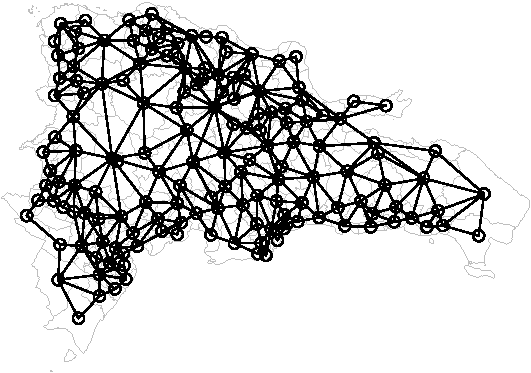
\includegraphics{proyecto_files/figure-latex/unnamed-chunk-3-1.pdf}

\begin{itemize}
\tightlist
\item
  En el análisis de vecinos más cercanos, JUAN DE HERRERA tiene un solo
  vecino y el que más tiene es la VEGA con 14 vecinos
\end{itemize}

\subsubsection{Pesos Espaciales}\label{pesos-espaciales}

\begin{itemize}
\tightlist
\item
  Los pesos que es la función para generar pesos en R utiliza el estilo
  denominado weighted o ``W'', se le asigno pesos usando criterios que
  elegimos en función de nuestro conocimiento del fenómeno analizado.
\end{itemize}

\begin{Shaded}
\begin{Highlighting}[]
\NormalTok{datosfuentes.w.W <-}\StringTok{ }\KeywordTok{nb2listw}\NormalTok{( datosfuentes.nb)}
\NormalTok{datosfuentes.w.W}
\end{Highlighting}
\end{Shaded}

\begin{verbatim}
## Characteristics of weights list object:
## Neighbour list object:
## Number of regions: 155 
## Number of nonzero links: 804 
## Percentage nonzero weights: 3.346514 
## Average number of links: 5.187097 
## 
## Weights style: W 
## Weights constants summary:
##     n    nn  S0       S1       S2
## W 155 24025 155 65.94606 650.7687
\end{verbatim}

\subsection{EDA para la Variable
seleccionada}\label{eda-para-la-variable-seleccionada}

\begin{Shaded}
\begin{Highlighting}[]
\NormalTok{coordsxy <-}\StringTok{ }\NormalTok{datosfuentes }\OperatorTok
\StringTok{  }\KeywordTok{st_centroid}\NormalTok{() }\OperatorTok\StringTok{ }
\StringTok{  }\KeywordTok{mutate}\NormalTok{(}\StringTok{"Pct Sabe leer y escribir: No sabe leer ni escribir"}\NormalTok{=}\StringTok{`}\DataTypeTok{Sabe leer y escribir: No sabe leer ni escribir}\StringTok{`}\OperatorTok{/}\NormalTok{(}\StringTok{`}\DataTypeTok{Población total}\StringTok{`}\NormalTok{)}\OperatorTok{*}\DecValTok{100}\NormalTok{,}
         \StringTok{"Pct Sabe leer y escribir: No sabe leer ni escribir log"}\NormalTok{=}\StringTok{ }\KeywordTok{log}\NormalTok{(}\StringTok{`}\DataTypeTok{Pct Sabe leer y escribir: No sabe leer ni escribir}\StringTok{`}\NormalTok{),}
         \DataTypeTok{x=}\KeywordTok{unlist}\NormalTok{(}\KeywordTok{map}\NormalTok{(geom,}\DecValTok{1}\NormalTok{)),}
         \DataTypeTok{y=}\KeywordTok{unlist}\NormalTok{(}\KeywordTok{map}\NormalTok{(geom,}\DecValTok{2}\NormalTok{))) }\OperatorTok
\StringTok{  }\KeywordTok{st_drop_geometry}\NormalTok{()}
\end{Highlighting}
\end{Shaded}

\begin{verbatim}
## Warning in st_centroid.sf(.): st_centroid assumes attributes are constant
## over geometries of x
\end{verbatim}

\begin{Shaded}
\begin{Highlighting}[]
\NormalTok{datosfuentes_sf <-}\StringTok{ }\NormalTok{datosfuentes }\OperatorTok
\StringTok{  }\KeywordTok{inner_join}\NormalTok{(coordsxy, }\DataTypeTok{by =} \StringTok{'TOPONIMIA'}\NormalTok{) }\OperatorTok\StringTok{ }
\StringTok{  }\NormalTok{dplyr}\OperatorTok{::}\KeywordTok{select}\NormalTok{(}\KeywordTok{matches}\NormalTok{(}\StringTok{'^Pct.*'}\NormalTok{), x, y, TOPONIMIA)}
\end{Highlighting}
\end{Shaded}

\subsection{EDA para No sabe leer ni
escribir}\label{eda-para-no-sabe-leer-ni-escribir}

\begin{Shaded}
\begin{Highlighting}[]
\NormalTok{p1 <-}\StringTok{ }\KeywordTok{tm_shape}\NormalTok{(datosfuentes_sf) }\OperatorTok{+}
\StringTok{  }\KeywordTok{tm_fill}\NormalTok{(}\DataTypeTok{col =} \StringTok{"Pct Sabe leer y escribir: No sabe leer ni escribir"}\NormalTok{, }\DataTypeTok{style =} \StringTok{'jenks'}\NormalTok{, }\DataTypeTok{palette =} \KeywordTok{brewer.pal}\NormalTok{(}\DecValTok{9}\NormalTok{, }\DataTypeTok{name =} \StringTok{'Reds'}\NormalTok{)) }\OperatorTok{+}
\StringTok{  }\KeywordTok{tm_borders}\NormalTok{(}\DataTypeTok{lwd =} \FloatTok{0.5}\NormalTok{)}
\NormalTok{p2 <-}\StringTok{ }\KeywordTok{tm_shape}\NormalTok{(datosfuentes_sf) }\OperatorTok{+}
\StringTok{  }\KeywordTok{tm_fill}\NormalTok{(}\DataTypeTok{col =} \StringTok{"Pct Sabe leer y escribir: No sabe leer ni escribir log"}\NormalTok{, }\DataTypeTok{style =} \StringTok{'jenks'}\NormalTok{,}
          \DataTypeTok{palette =} \KeywordTok{brewer.pal}\NormalTok{(}\DecValTok{9}\NormalTok{, }\DataTypeTok{name =} \StringTok{'Reds'}\NormalTok{), }\DataTypeTok{midpoint =} \OtherTok{NA}\NormalTok{) }\OperatorTok{+}
\StringTok{  }\KeywordTok{tm_borders}\NormalTok{(}\DataTypeTok{lwd =} \FloatTok{0.5}\NormalTok{)}
\KeywordTok{tmap_arrange}\NormalTok{(p1, p2)}
\end{Highlighting}
\end{Shaded}

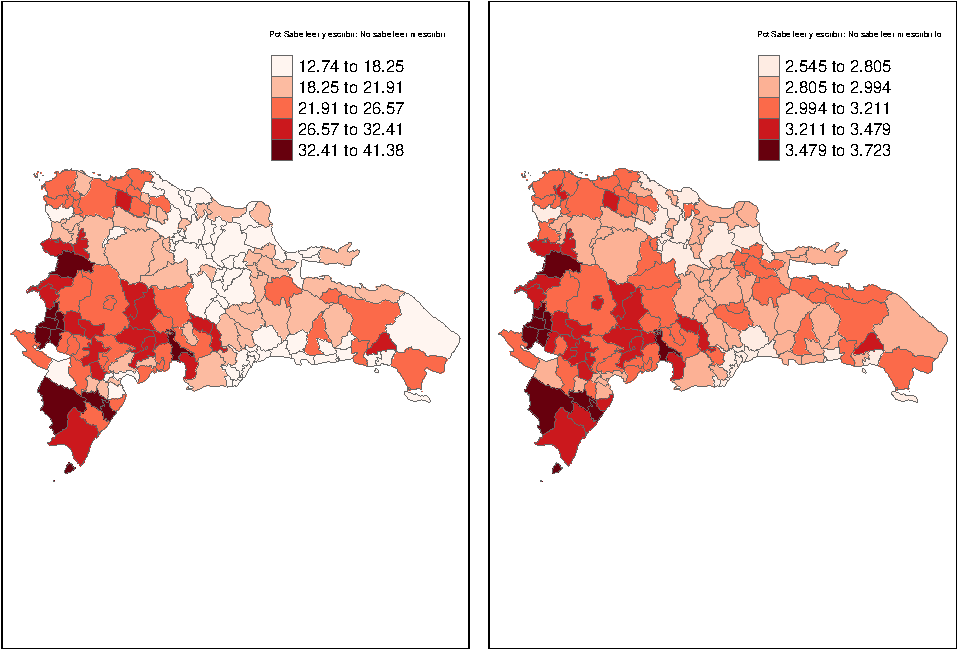
\includegraphics{proyecto_files/figure-latex/unnamed-chunk-6-1.pdf}

\begin{itemize}
\item
  Según el análisis exploratorio de los datos podemos ver en el mapa de
  la variable original que hay 54 municipios con aproximadamente 15\% de
  personas que no saben leer ni escribir, 42 con un aproximado de 20\%
  de personas que no sabe leer ni escribir, 34 municipios con un
  aproximado de 24\% de personas que no sabe leer ni escribir, 20
  municipios de aproximadamente 29\% de personas que no sabe leer ni
  escribir y 6 de los municipios tiene un 37\% con un alto porcentaje
  que no sabe leer ni escribir.
\item
  En el análisis exploratorio de los datos podemos ver en el mapa de la
  variable logarítmica que hay 24 municipios con aproximadamente 3\% de
  personas que no saben leer ni escribir, 51 municipios con un
  aproximado de 3\% de personas que no sabe leer ni escribir, 48
  municipios con un aproximado de 3\% de personas que no sabe leer ni
  escribir, 27 municipios con aproximadamente 3\% de las personas no
  sabe leer ni escribir y 5 municipios de aproximadamente 4\% de las
  personas no sabe leer ni escribir
\end{itemize}

\subsubsection{Crear Diagrama Cuantilar
Normal}\label{crear-diagrama-cuantilar-normal}

\begin{Shaded}
\begin{Highlighting}[]
\NormalTok{ datosfuentes_sf }\OperatorTok\StringTok{ }\KeywordTok{st_drop_geometry}\NormalTok{() }\OperatorTok
\StringTok{  }\KeywordTok{gather}\NormalTok{(variable, valor, }\OperatorTok{-}\NormalTok{(x}\OperatorTok{:}\NormalTok{TOPONIMIA)) }\OperatorTok
\StringTok{  }\KeywordTok{ggplot}\NormalTok{() }\OperatorTok{+}\StringTok{ }\KeywordTok{aes}\NormalTok{(}\DataTypeTok{sample=}\NormalTok{valor) }\OperatorTok{+}
\StringTok{  }\KeywordTok{stat_qq}\NormalTok{() }\OperatorTok{+}\StringTok{ }\KeywordTok{stat_qq_line}\NormalTok{() }\OperatorTok{+}\StringTok{ }\KeywordTok{theme_bw}\NormalTok{() }\OperatorTok{+}
\StringTok{  }\KeywordTok{theme}\NormalTok{(}\DataTypeTok{text =} \KeywordTok{element_text}\NormalTok{(}\DataTypeTok{size =} \DecValTok{14}\NormalTok{)) }\OperatorTok{+}
\StringTok{  }\KeywordTok{facet_wrap}\NormalTok{(}\OperatorTok{~}\NormalTok{variable, }\DataTypeTok{scales =} \StringTok{'free'}\NormalTok{)}
\end{Highlighting}
\end{Shaded}

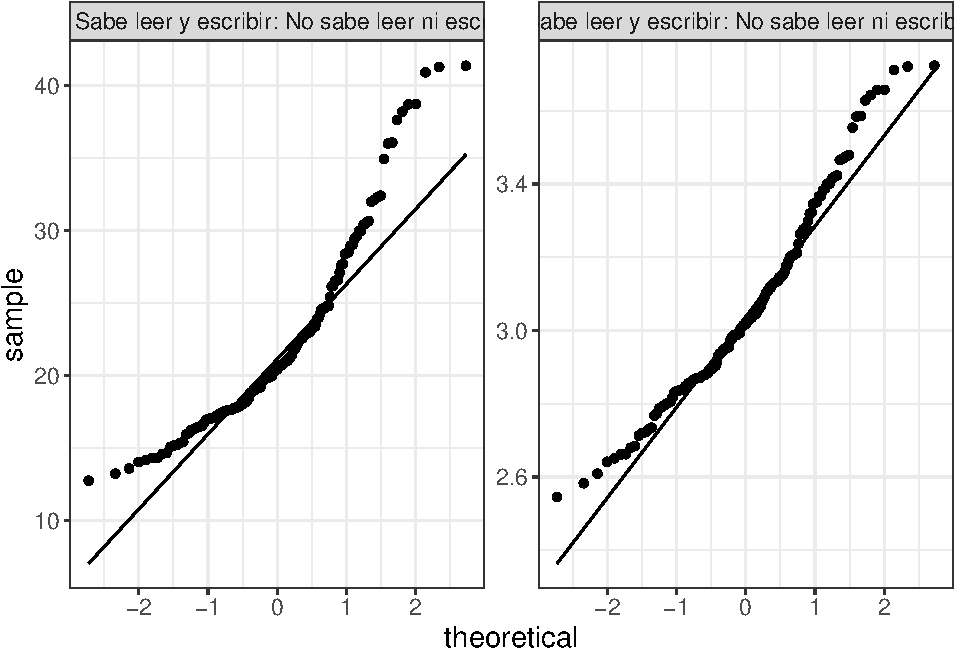
\includegraphics{proyecto_files/figure-latex/unnamed-chunk-7-1.pdf}

\begin{itemize}
\tightlist
\item
  Según el diagrama cuantilar normal, la gráfica logarítmica presenta
  más normalidad en los datos, ya que se asemeja más a una línea recta
\end{itemize}

\subsubsection{Prueba de Shapiro-Wilk}\label{prueba-de-shapiro-wilk-1}

\begin{Shaded}
\begin{Highlighting}[]
\NormalTok{datosfuentes_sf }\OperatorTok\StringTok{ }\KeywordTok{st_drop_geometry}\NormalTok{() }\OperatorTok
\StringTok{  }\KeywordTok{gather}\NormalTok{(variable, valor, }\OperatorTok{-}\NormalTok{(x}\OperatorTok{:}\NormalTok{TOPONIMIA)) }\OperatorTok\StringTok{ }\KeywordTok{group_by}\NormalTok{(variable) }\OperatorTok
\StringTok{  }\KeywordTok{summarise}\NormalTok{(}\DataTypeTok{prueba_normalidad=}\KeywordTok{shapiro.test}\NormalTok{(valor)}\OperatorTok{$}\NormalTok{p.value)}
\end{Highlighting}
\end{Shaded}

\begin{verbatim}
## # A tibble: 2 x 2
##   variable                                               prueba_normalidad
##   <chr>                                                              <dbl>
## 1 Pct Sabe leer y escribir: No sabe leer ni escribir         0.00000000512
## 2 Pct Sabe leer y escribir: No sabe leer ni escribir log     0.000550
\end{verbatim}

\begin{itemize}
\tightlist
\item
  Para la prueba de Shapiro-Wilk al menos los datos transformados, sí
  cumplen en principio con el supuesto de normalidad.
\end{itemize}

\subsubsection{Comprobacion de
Homocedasticidad}\label{comprobacion-de-homocedasticidad-1}

\begin{Shaded}
\begin{Highlighting}[]
\NormalTok{datosfuentes_sf }\OperatorTok\StringTok{ }\KeywordTok{lm}\NormalTok{(}\StringTok{`}\DataTypeTok{Pct Sabe leer y escribir: No sabe leer ni escribir log}\StringTok{`}\OperatorTok{~}\StringTok{ }\NormalTok{x, .) }\OperatorTok\StringTok{ }\KeywordTok{plot}\NormalTok{(}\DecValTok{3}\NormalTok{)}
\end{Highlighting}
\end{Shaded}

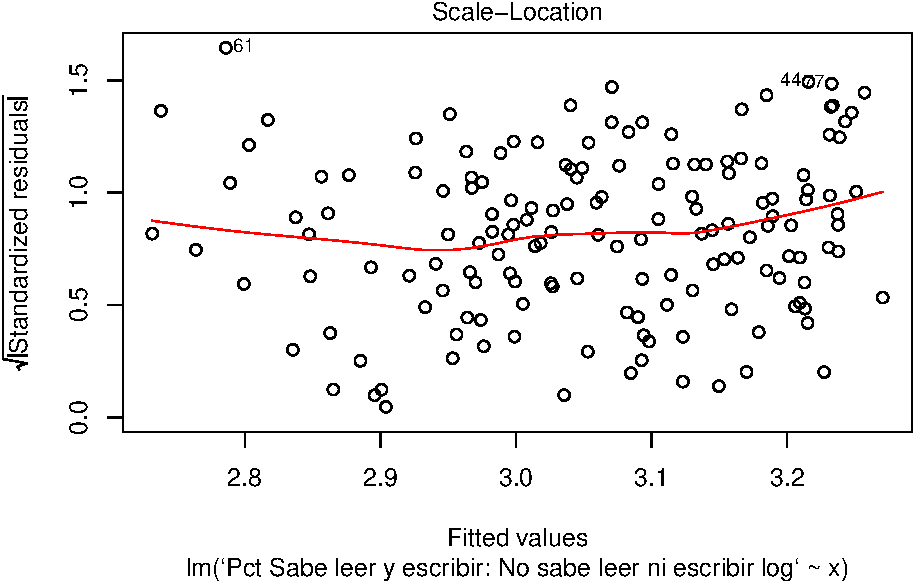
\includegraphics{proyecto_files/figure-latex/unnamed-chunk-9-1.pdf}

\begin{Shaded}
\begin{Highlighting}[]
\NormalTok{datosfuentes_sf }\OperatorTok\StringTok{ }\KeywordTok{lm}\NormalTok{(}\StringTok{`}\DataTypeTok{Pct Sabe leer y escribir: No sabe leer ni escribir log}\StringTok{`}\OperatorTok{~}\StringTok{ }\NormalTok{y, .) }\OperatorTok\StringTok{ }\KeywordTok{plot}\NormalTok{(}\DecValTok{3}\NormalTok{)}
\end{Highlighting}
\end{Shaded}

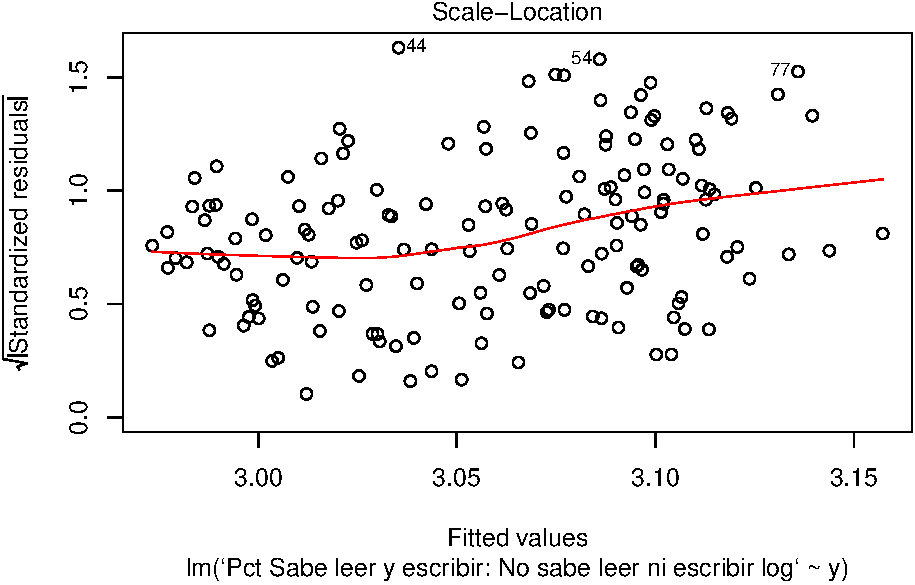
\includegraphics{proyecto_files/figure-latex/unnamed-chunk-9-2.pdf}

\begin{Shaded}
\begin{Highlighting}[]
\NormalTok{datosfuentes_sf }\OperatorTok\StringTok{ }\KeywordTok{lm}\NormalTok{(}\StringTok{`}\DataTypeTok{Pct Sabe leer y escribir: No sabe leer ni escribir log}\StringTok{`}\OperatorTok{~}\StringTok{ }\NormalTok{y, .) }\OperatorTok\StringTok{ }\KeywordTok{bptest}\NormalTok{()}
\end{Highlighting}
\end{Shaded}

\begin{verbatim}
## 
##  studentized Breusch-Pagan test
## 
## data:  .
## BP = 12.689, df = 1, p-value = 0.0003677
\end{verbatim}

\begin{Shaded}
\begin{Highlighting}[]
\NormalTok{datosfuentes_sf }\OperatorTok\StringTok{ }\KeywordTok{lm}\NormalTok{(}\StringTok{`}\DataTypeTok{Pct Sabe leer y escribir: No sabe leer ni escribir log}\StringTok{`}\OperatorTok{~}\StringTok{ }\NormalTok{x, .) }\OperatorTok\StringTok{ }\KeywordTok{bptest}\NormalTok{()}
\end{Highlighting}
\end{Shaded}

\begin{verbatim}
## 
##  studentized Breusch-Pagan test
## 
## data:  .
## BP = 0.97226, df = 1, p-value = 0.3241
\end{verbatim}

\begin{itemize}
\tightlist
\item
  Según la comprobación de homocedasticidad, para la variable respecto
  de la coordenada Y, tanto grafico como la prueba de homocedasticidad,
  el resultado obtenido sugiere heterocedasticidad. Pero respecto de X
  hay homocedasticidad.
\end{itemize}

\subsection{Evaluar la Autocorrelacion Espacial
Global}\label{evaluar-la-autocorrelacion-espacial-global-1}

\begin{Shaded}
\begin{Highlighting}[]
\NormalTok{(gmoranw <-}\StringTok{ }\KeywordTok{moran.test}\NormalTok{(}\DataTypeTok{x =}\NormalTok{ datosfuentes_sf}\OperatorTok{$}\StringTok{`}\DataTypeTok{Pct Sabe leer y escribir: No sabe leer ni escribir log}\StringTok{`}\NormalTok{, }\DataTypeTok{listw =}\NormalTok{ datosfuentes.w.W))}
\end{Highlighting}
\end{Shaded}

\begin{verbatim}
## 
##  Moran I test under randomisation
## 
## data:  datosfuentes_sf$`Pct Sabe leer y escribir: No sabe leer ni escribir log`  
## weights: datosfuentes.w.W    
## 
## Moran I statistic standard deviate = 11.835, p-value < 2.2e-16
## alternative hypothesis: greater
## sample estimates:
## Moran I statistic       Expectation          Variance 
##       0.603141844      -0.006493506       0.002653516
\end{verbatim}

\begin{itemize}
\tightlist
\item
  En esta investigación se rechaza la hipótesis nula, porque el
  coeficiente de significancia es menor que 0.05
\end{itemize}

\subsection{Evaluar la Autocorrelacion Espacial
Local}\label{evaluar-la-autocorrelacion-espacial-local}

\subsubsection{Prueba de I Moran Local}\label{prueba-de-i-moran-local-1}

\begin{Shaded}
\begin{Highlighting}[]
\KeywordTok{moran.plot}\NormalTok{(}\DataTypeTok{x =}\NormalTok{ datosfuentes_sf}\OperatorTok{$}\StringTok{`}\DataTypeTok{Pct Sabe leer y escribir: No sabe leer ni escribir log}\StringTok{`}\NormalTok{, }\DataTypeTok{listw =}\NormalTok{ datosfuentes.w.W)}
\end{Highlighting}
\end{Shaded}

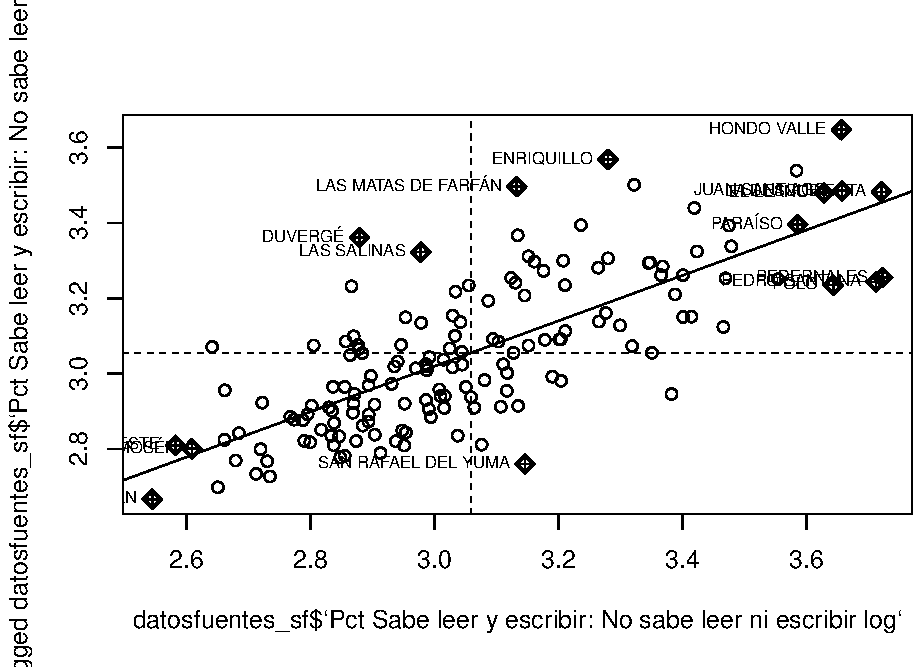
\includegraphics{proyecto_files/figure-latex/unnamed-chunk-11-1.pdf}

\begin{itemize}
\tightlist
\item
  En el diagrama de Moran Plot San Rafael del Yuma, tiene un valor de la
  variable en el eje X de 3.2, en el eje Y de acuerdo a su vecindad se
  esperaría de 2.8, San Rafael del Yuma tiene mucha más población que no
  sabe leer ni escribir, que lo que se esperaría de acuerdo a su
  entorno, eso se considera un outlayer espacial o un aberración
  espacial. En San Rafael del Yuma se observó un valor grande, pero se
  espera un valor más pequeño. Duvergé es un caso contrario, se obtiene
  un valor de la variable de 2.9, pero de acuerdo a su vecindad, Duvergé
  se esperaría es 3.4, se esperaría un analfabetismo grande, pero se
  obtuvo un valor menor.
\end{itemize}

\subsubsection{Generar Mapa Clusters
lisa}\label{generar-mapa-clusters-lisa}

\begin{Shaded}
\begin{Highlighting}[]
\KeywordTok{lisamap}\NormalTok{(}\DataTypeTok{objesp =}\NormalTok{ datosfuentes_sf,}
        \DataTypeTok{var =} \StringTok{'Pct Sabe leer y escribir: No sabe leer ni escribir log'}\NormalTok{,}
        \DataTypeTok{pesos =}\NormalTok{ datosfuentes.w.W,}
        \DataTypeTok{tituloleyenda =} \StringTok{'Significancia}\CharTok{\textbackslash{}n}\StringTok{("x-y", léase}\CharTok{\textbackslash{}n}\StringTok{como "x"}\CharTok{\textbackslash{}n}\StringTok{rodeado de "y"'}\NormalTok{,}
        \DataTypeTok{leyenda =}\NormalTok{ T,}
        \DataTypeTok{anchuratitulo =} \DecValTok{100}\NormalTok{,}
        \DataTypeTok{tamanotitulo =} \DecValTok{16}\NormalTok{,}
        \DataTypeTok{fuentedatos =} \StringTok{'ENHOGAR 2017'}\NormalTok{,}
        \DataTypeTok{titulomapa =} \KeywordTok{paste0}\NormalTok{(}\StringTok{'Clusters LISA de respuestas a la pregunta:}\CharTok{\textbackslash{}n}\StringTok{"'}\NormalTok{,}\StringTok{"Pct Sabe leer y escribir: No sabe leer ni escribir log"}\NormalTok{ , }\StringTok{'"'}\NormalTok{))}
\end{Highlighting}
\end{Shaded}

\begin{verbatim}
## $grafico
\end{verbatim}

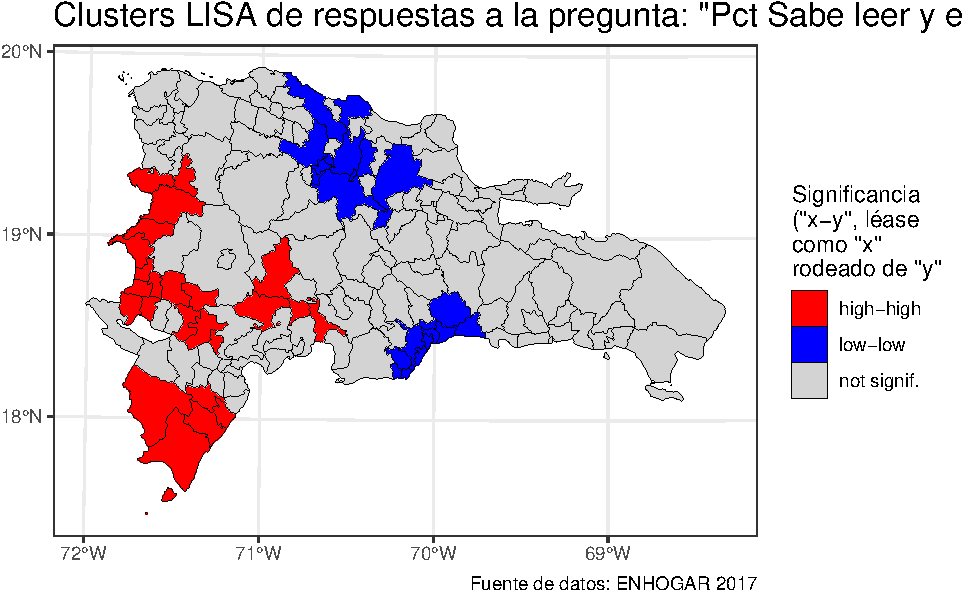
\includegraphics{proyecto_files/figure-latex/unnamed-chunk-12-1.pdf}

\begin{verbatim}
## 
## $objeto
## Simple feature collection with 155 features and 8 fields
## geometry type:  MULTIPOLYGON
## dimension:      XY
## bbox:           xmin: 182215.8 ymin: 1933532 xmax: 571365.3 ymax: 2205216
## epsg (SRID):    32619
## proj4string:    +proj=utm +zone=19 +datum=WGS84 +units=m +no_defs
## First 10 features:
##    Pct Sabe leer y escribir: No sabe leer ni escribir
## 1                                            12.74486
## 2                                            22.72702
## 3                                            29.60064
## 4                                            28.37117
## 5                                            32.11417
## 6                                            32.41135
## 7                                            21.23028
## 8                                            23.99644
## 9                                            29.98810
## 10                                           22.97169
##    Pct Sabe leer y escribir: No sabe leer ni escribir log        x       y
## 1                                                2.545128 400576.8 2044091
## 2                                                3.123555 308829.1 2037708
## 3                                                3.387796 336675.2 2034232
## 4                                                3.345373 289007.6 2058192
## 5                                                3.469297 298570.6 2080773
## 6                                                3.478509 311899.8 2057722
## 7                                                3.055429 300563.9 2037000
## 8                                                3.177905 311931.4 2034599
## 9                                                3.400801 297803.0 2046138
## 10                                               3.134263 313902.6 2070484
##                  TOPONIMIA                           geom puntuacionz
## 1  SANTO DOMINGO DE GUZMÁN MULTIPOLYGON (((405218.1 20... -1.98817365
## 2                     AZUA MULTIPOLYGON (((319065.3 20...  0.24918591
## 3              LAS CHARCAS MULTIPOLYGON (((341415.3 20...  1.27127372
## 4     LAS YAYAS DE VIAJAMA MULTIPOLYGON (((304058.1 20...  1.10718295
## 5          PADRE LAS CASAS MULTIPOLYGON (((312890.8 20...  1.58652129
## 6                  PERALTA MULTIPOLYGON (((317370.6 20...  1.62215145
## 7             SABANA YEGUA MULTIPOLYGON (((306745.8 20... -0.01432628
## 8             PUEBLO VIEJO MULTIPOLYGON (((310447.9 20...  0.45941522
## 9            TÁBARA ARRIBA MULTIPOLYGON (((306556.7 20...  1.32157579
## 10                GUAYABAL MULTIPOLYGON (((322129.5 20...  0.29060399
##    lagpuntuacionz    quad_sig
## 1      -1.5183907     low-low
## 2       0.7535335 not signif.
## 3       0.5844024 not signif.
## 4       0.9071218   high-high
## 5       0.7495699   high-high
## 6       1.0780923   high-high
## 7       0.6767256 not signif.
## 8       0.1174298 not signif.
## 9       0.3527162 not signif.
## 10      1.1915914 not signif.
\end{verbatim}

\begin{itemize}
\tightlist
\item
  El Mapa LISA Cliusters, nos muestra cuales son los grumos o
  aglomerados del valor alto de la variable, el valor alto de la
  variable es el porcentaje de persona que no sabe leer ni escribir, esa
  variable se comporta de la manera grumosa en 24 municipio, entre estos
  están: la región Enriquillo en una parte de ella y en esos municipio y
  en algunos municipios de la región fronteriza y también al norte de la
  provincia de Azua, eso son los aglomerados donde los municipios de ese
  grumo se parecen a su entorno en cuanto a esa variable, es decir
  Pedernales se parece a Oviedo, Oviedo se parece a Paraíso, entre sí en
  cuanto al valor de la variable, es decir están autocorrelacionado
  espacialmente en cuanto a esa variable. En 23 municipios pasa el
  efecto contrario estos municipios están autorrelacionado entre sí pero
  con bajo valor de la variable, la variable tiene un bajo valor en
  Santo Domingo, San Cristóbal, Santo Domingo Norte, entre otros.
  Existen Dos grumos de bajo valor de las variables y tres grumos de
  alto valor de las variables. En el recto como no se parece entre sí,
  no hay una autocorrelacion espacial entre ellos, no hay una
  auotcorrelacion significativa y por eso se ponen todos de color gris.
\end{itemize}

\subsection{Modelización de datos
espaciales}\label{modelizaciuxf3n-de-datos-espaciales-1}

\subsubsection{Selección de variables}\label{selecciuxf3n-de-variables}

\begin{itemize}
\item
  Dentro del proyecto de investigación voy a trabajar con la
  modelización de datos espaciales para ello esta, el grado de
  asociación de diferentes variables, dende se encuentra la principal
  como ``sabe leer y escribir: No sabe leer ni escribir''.
\item
  Sabe leer y escribir: No sabe leer ni escribir
\item
  Población total
\item
  Tipo de vivienda: Pieza en cuartería o parte atrás
\item
  Tipo de vivienda: Barracón
\item
  Edad en grupos quinquenales 0, 1-4, \ldots{}. 85 y más: 60 - 64
\item
  Condición Actividad Económica: Trabajador(a) familiar o no familiar
  sin paga o ganancia
\item
  Asiste o asistió a la escuela: No asiste, pero asistió
\end{itemize}

\subsection{Cargar Datos}\label{cargar-datos-1}

\begin{itemize}
\tightlist
\item
  Vamos hacer las selecciones correspondientes y a las variables le
  atribuimos nombres cortos, conservando el campo ENLACE y TOPONIMIA:
\end{itemize}

\begin{Shaded}
\begin{Highlighting}[]
\NormalTok{alfa <-}\StringTok{ }\NormalTok{datosfuentes }\OperatorTok\StringTok{ }\NormalTok{dplyr}\OperatorTok{::}\KeywordTok{select}\NormalTok{(}
  \DataTypeTok{ENLACE =}\NormalTok{ ENLACE,}
  \DataTypeTok{TOPONIMIA =}\NormalTok{ TOPONIMIA,}
  \DataTypeTok{POBLA=} \StringTok{`}\DataTypeTok{Población total}\StringTok{`}\NormalTok{,}
  \DataTypeTok{VICUARTERIA =} \StringTok{`}\DataTypeTok{Tipo de vivienda: Pieza en cuartería o parte atrás}\StringTok{`}\NormalTok{,}
  \DataTypeTok{VIBARRACON =} \StringTok{`}\DataTypeTok{Tipo de vivienda: Barracón`,}
\DataTypeTok{  TERCERAEDAD = }\StringTok{`}\NormalTok{Edad en grupos quinquenales }\DecValTok{0}\NormalTok{, }\DecValTok{1}\OperatorTok{-}\DecValTok{4}\NormalTok{, .... }\DecValTok{85}\NormalTok{ y más}\OperatorTok{:}\StringTok{ }\DecValTok{60} \OperatorTok{-}\StringTok{ }\DecValTok{64}\StringTok{`}\DataTypeTok{,}
\DataTypeTok{  TRASINPAGA = }\StringTok{`}\NormalTok{Condición Actividad Económica: }\KeywordTok{Trabajador}\NormalTok{(a) familiar o no familiar sin paga o ganancia}\StringTok{`}\DataTypeTok{,}
\DataTypeTok{  ASISTIOESC = }\StringTok{`}\NormalTok{Asiste o asistió a la escuela}\OperatorTok{:}\StringTok{ }\NormalTok{No asiste, pero asistió`,}
  \DataTypeTok{ANALFABETISMO=} \StringTok{`}\DataTypeTok{Sabe leer y escribir: No sabe leer ni escribir}\StringTok{`}\NormalTok{)}
\NormalTok{alfa}
\end{Highlighting}
\end{Shaded}

\begin{verbatim}
## Simple feature collection with 155 features and 9 fields
## geometry type:  MULTIPOLYGON
## dimension:      XY
## bbox:           xmin: 182215.8 ymin: 1933532 xmax: 571365.3 ymax: 2205216
## epsg (SRID):    32619
## proj4string:    +proj=utm +zone=19 +datum=WGS84 +units=m +no_defs
## First 10 features:
##    ENLACE               TOPONIMIA  POBLA VICUARTERIA VIBARRACON
## 1  100101 SANTO DOMINGO DE GUZMÁN 965040       27922        587
## 2  050201                    AZUA  91345        1683         48
## 3  050202             LAS CHARCAS  11243         296          4
## 4  050203    LAS YAYAS DE VIAJAMA  17620         283         10
## 5  050204         PADRE LAS CASAS  20041          56          1
## 6  050205                 PERALTA  15257          78          3
## 7  050206            SABANA YEGUA  19020         282          2
## 8  050207            PUEBLO VIEJO  11235          26          2
## 9  050208           TÁBARA ARRIBA  17647          35         14
## 10 050209                GUAYABAL   5263          44          0
##    TERCERAEDAD TRASINPAGA ASISTIOESC ANALFABETISMO
## 1        31976       6201     514540        122993
## 2         2559        990      40563         20760
## 3          325         84       5128          3328
## 4          567        356       7281          4999
## 5          635        429       7831          6436
## 6          402        259       6412          4945
## 7          541        404       8863          4038
## 8          286        160       5016          2696
## 9          559        305       7390          5292
## 10         167        158       2043          1209
##                              geom
## 1  MULTIPOLYGON (((405218.1 20...
## 2  MULTIPOLYGON (((319065.3 20...
## 3  MULTIPOLYGON (((341415.3 20...
## 4  MULTIPOLYGON (((304058.1 20...
## 5  MULTIPOLYGON (((312890.8 20...
## 6  MULTIPOLYGON (((317370.6 20...
## 7  MULTIPOLYGON (((306745.8 20...
## 8  MULTIPOLYGON (((310447.9 20...
## 9  MULTIPOLYGON (((306556.7 20...
## 10 MULTIPOLYGON (((322129.5 20...
\end{verbatim}

\subsubsection{Relativizar}\label{relativizar}

\begin{itemize}
\tightlist
\item
  Vamos a relativizar todas las columnas numéricas con el campo POBLA,
  generando así nuevas columnas de porcentaje (nombre de columnas con
  sufijo \_PCT). Al mismo tiempo, obtendremos los logaritmos de la base,
  de los porcentajes (nombre de columnas con sufijo \_PCTLOG).
\end{itemize}

\begin{Shaded}
\begin{Highlighting}[]
\NormalTok{alfapctlog <-}\StringTok{ }\NormalTok{alfa }\OperatorTok\StringTok{ }\KeywordTok{mutate_each}\NormalTok{(}
  \KeywordTok{funs}\NormalTok{(}\DataTypeTok{PCT=}\KeywordTok{round}\NormalTok{(.}\OperatorTok{/}\NormalTok{POBLA,}\DecValTok{4}\NormalTok{)}\OperatorTok{*}\DecValTok{100}\NormalTok{,}
       \DataTypeTok{PCTLOG=}\KeywordTok{log1p}\NormalTok{(}\KeywordTok{round}\NormalTok{(.}\OperatorTok{/}\NormalTok{POBLA,}\DecValTok{4}\NormalTok{)}\OperatorTok{*}\DecValTok{100}\NormalTok{)),}
  \OperatorTok{-}\DecValTok{1}\NormalTok{, }\OperatorTok{-}\DecValTok{2}\NormalTok{, }\OperatorTok{-}\NormalTok{geom, }\OperatorTok{-}\NormalTok{POBLA)}
\end{Highlighting}
\end{Shaded}

\begin{verbatim}
## Warning: funs() is soft deprecated as of dplyr 0.8.0
## Please use a list of either functions or lambdas: 
## 
##   # Simple named list: 
##   list(mean = mean, median = median)
## 
##   # Auto named with `tibble::lst()`: 
##   tibble::lst(mean, median)
## 
##   # Using lambdas
##   list(~ mean(., trim = .2), ~ median(., na.rm = TRUE))
## This warning is displayed once per session.
\end{verbatim}

\begin{Shaded}
\begin{Highlighting}[]
\NormalTok{alfapctlog}
\end{Highlighting}
\end{Shaded}

\begin{verbatim}
## Simple feature collection with 155 features and 21 fields
## geometry type:  MULTIPOLYGON
## dimension:      XY
## bbox:           xmin: 182215.8 ymin: 1933532 xmax: 571365.3 ymax: 2205216
## epsg (SRID):    32619
## proj4string:    +proj=utm +zone=19 +datum=WGS84 +units=m +no_defs
## First 10 features:
##    ENLACE               TOPONIMIA  POBLA VICUARTERIA VIBARRACON
## 1  100101 SANTO DOMINGO DE GUZMÁN 965040       27922        587
## 2  050201                    AZUA  91345        1683         48
## 3  050202             LAS CHARCAS  11243         296          4
## 4  050203    LAS YAYAS DE VIAJAMA  17620         283         10
## 5  050204         PADRE LAS CASAS  20041          56          1
## 6  050205                 PERALTA  15257          78          3
## 7  050206            SABANA YEGUA  19020         282          2
## 8  050207            PUEBLO VIEJO  11235          26          2
## 9  050208           TÁBARA ARRIBA  17647          35         14
## 10 050209                GUAYABAL   5263          44          0
##    TERCERAEDAD TRASINPAGA ASISTIOESC ANALFABETISMO
## 1        31976       6201     514540        122993
## 2         2559        990      40563         20760
## 3          325         84       5128          3328
## 4          567        356       7281          4999
## 5          635        429       7831          6436
## 6          402        259       6412          4945
## 7          541        404       8863          4038
## 8          286        160       5016          2696
## 9          559        305       7390          5292
## 10         167        158       2043          1209
##                              geom VICUARTERIA_PCT VIBARRACON_PCT
## 1  MULTIPOLYGON (((405218.1 20...            2.89           0.06
## 2  MULTIPOLYGON (((319065.3 20...            1.84           0.05
## 3  MULTIPOLYGON (((341415.3 20...            2.63           0.04
## 4  MULTIPOLYGON (((304058.1 20...            1.61           0.06
## 5  MULTIPOLYGON (((312890.8 20...            0.28           0.00
## 6  MULTIPOLYGON (((317370.6 20...            0.51           0.02
## 7  MULTIPOLYGON (((306745.8 20...            1.48           0.01
## 8  MULTIPOLYGON (((310447.9 20...            0.23           0.02
## 9  MULTIPOLYGON (((306556.7 20...            0.20           0.08
## 10 MULTIPOLYGON (((322129.5 20...            0.84           0.00
##    TERCERAEDAD_PCT TRASINPAGA_PCT ASISTIOESC_PCT ANALFABETISMO_PCT
## 1             3.31           0.64          53.32             12.74
## 2             2.80           1.08          44.41             22.73
## 3             2.89           0.75          45.61             29.60
## 4             3.22           2.02          41.32             28.37
## 5             3.17           2.14          39.07             32.11
## 6             2.63           1.70          42.03             32.41
## 7             2.84           2.12          46.60             21.23
## 8             2.55           1.42          44.65             24.00
## 9             3.17           1.73          41.88             29.99
## 10            3.17           3.00          38.82             22.97
##    VICUARTERIA_PCTLOG VIBARRACON_PCTLOG TERCERAEDAD_PCTLOG
## 1           1.3584092       0.058268908           1.460938
## 2           1.0438041       0.048790164           1.335001
## 3           1.2892326       0.039220713           1.358409
## 4           0.9593502       0.058268908           1.439835
## 5           0.2468601       0.000000000           1.427916
## 6           0.4121097       0.019802627           1.289233
## 7           0.9082586       0.009950331           1.345472
## 8           0.2070142       0.019802627           1.266948
## 9           0.1823216       0.076961041           1.427916
## 10          0.6097656       0.000000000           1.427916
##    TRASINPAGA_PCTLOG ASISTIOESC_PCTLOG ANALFABETISMO_PCTLOG
## 1          0.4946962          3.994892             2.620311
## 2          0.7323679          3.815732             3.166740
## 3          0.5596158          3.841815             3.421000
## 4          1.1052568          3.745260             3.379974
## 5          1.1442228          3.690628             3.499835
## 6          0.9932518          3.761898             3.508855
## 7          1.1378330          3.862833             3.101443
## 8          0.8837675          3.821004             3.218876
## 9          1.0043016          3.758406             3.433665
## 10         1.3862944          3.684369             3.176803
\end{verbatim}

\subsubsection{Modelo Lineal}\label{modelo-lineal}

\begin{Shaded}
\begin{Highlighting}[]
\NormalTok{modlin <-}\StringTok{ }\NormalTok{alfapctlog }\OperatorTok\StringTok{ }\KeywordTok{select}\NormalTok{(}\KeywordTok{contains}\NormalTok{(}\StringTok{'_PCTLOG'}\NormalTok{)) }\OperatorTok
\StringTok{  }\KeywordTok{st_drop_geometry}\NormalTok{() }\OperatorTok\StringTok{ }\KeywordTok{lm}\NormalTok{(ANALFABETISMO_PCTLOG }\OperatorTok{~}\StringTok{ }\NormalTok{., .)}
\NormalTok{modlin }\OperatorTok\StringTok{ }\NormalTok{summary}
\end{Highlighting}
\end{Shaded}

\begin{verbatim}
## 
## Call:
## lm(formula = ANALFABETISMO_PCTLOG ~ ., data = .)
## 
## Residuals:
##      Min       1Q   Median       3Q      Max 
## -0.29529 -0.09118 -0.01235  0.07643  0.42540 
## 
## Coefficients:
##                    Estimate Std. Error t value Pr(>|t|)    
## (Intercept)         7.29304    0.31061  23.480  < 2e-16 ***
## VICUARTERIA_PCTLOG  0.02398    0.03268   0.734   0.4643    
## VIBARRACON_PCTLOG   0.04547    0.03004   1.514   0.1322    
## TERCERAEDAD_PCTLOG  0.43638    0.10081   4.329 2.74e-05 ***
## TRASINPAGA_PCTLOG   0.13983    0.05400   2.589   0.0106 *  
## ASISTIOESC_PCTLOG  -1.28148    0.07426 -17.258  < 2e-16 ***
## ---
## Signif. codes:  0 '***' 0.001 '**' 0.01 '*' 0.05 '.' 0.1 ' ' 1
## 
## Residual standard error: 0.1305 on 149 degrees of freedom
## Multiple R-squared:  0.7309, Adjusted R-squared:  0.7218 
## F-statistic: 80.92 on 5 and 149 DF,  p-value: < 2.2e-16
\end{verbatim}

\subsubsection{Modelo Espacial
Autorregresivo}\label{modelo-espacial-autorregresivo-1}

\paragraph{Modelo con todas
Variables}\label{modelo-con-todas-variables-1}

\begin{Shaded}
\begin{Highlighting}[]
\NormalTok{sar <-}\StringTok{ }\NormalTok{alfapctlog }\OperatorTok\StringTok{ }\KeywordTok{select}\NormalTok{(}\KeywordTok{contains}\NormalTok{(}\StringTok{'_PCTLOG'}\NormalTok{)) }\OperatorTok
\StringTok{  }\KeywordTok{st_drop_geometry}\NormalTok{() }\OperatorTok
\StringTok{  }\KeywordTok{spautolm}\NormalTok{(}
    \DataTypeTok{formula =}\NormalTok{ ANALFABETISMO_PCTLOG }\OperatorTok{~}\StringTok{ }\NormalTok{.,}
    \DataTypeTok{data =}\NormalTok{ .,}
    \DataTypeTok{listw =}\NormalTok{ datosfuentes.w.W)}
\KeywordTok{summary}\NormalTok{(sar)}
\end{Highlighting}
\end{Shaded}

\begin{verbatim}
## 
## Call: 
## spautolm(formula = ANALFABETISMO_PCTLOG ~ ., data = ., listw = datosfuentes.w.W)
## 
## Residuals:
##        Min         1Q     Median         3Q        Max 
## -0.3402646 -0.0605722 -0.0026683  0.0672125  0.3338405 
## 
## Coefficients: 
##                     Estimate Std. Error  z value  Pr(>|z|)
## (Intercept)         7.710569   0.379417  20.3221 < 2.2e-16
## VICUARTERIA_PCTLOG -0.037173   0.026782  -1.3880  0.165135
## VIBARRACON_PCTLOG   0.071284   0.027405   2.6011  0.009293
## TERCERAEDAD_PCTLOG  0.259888   0.087802   2.9599  0.003077
## TRASINPAGA_PCTLOG   0.053992   0.045566   1.1849  0.236051
## ASISTIOESC_PCTLOG  -1.297447   0.094929 -13.6676 < 2.2e-16
## 
## Lambda: 0.67854 LR test value: 52.748 p-value: 3.7914e-13 
## Numerical Hessian standard error of lambda: 0.070969 
## 
## Log likelihood: 125.0939 
## ML residual variance (sigma squared): 0.010353, (sigma: 0.10175)
## Number of observations: 155 
## Number of parameters estimated: 8 
## AIC: -234.19
\end{verbatim}

\begin{itemize}
\tightlist
\item
  En los casos de las variables, Tipo de vivienda:
  Barracón\texttt{,}Edad en grupos quinquenales 0, 1-4,\ldots{}. 85 y
  más: 60 - 64\texttt{,}Asiste o asistió a la escuela: No asiste, pero
  asistió\texttt{,\ están\ asociada\ porque\ presentan\ coeficientes\ significativos\ y}Tipo
  de vivienda: Pieza en cuartería o parte atrás\texttt{,}Condición
  Actividad Económica: Trabajador(a) familiar o no familiar sin paga o
  ganancia`, no están asociado porque presentan coeficiente no
  significativo.
\end{itemize}

\paragraph{Modelo con Variables cuyo Coeficientes Resultaron
Significativo}\label{modelo-con-variables-cuyo-coeficientes-resultaron-significativo-1}

\begin{Shaded}
\begin{Highlighting}[]
\NormalTok{sar2 <-}\StringTok{ }\NormalTok{alfapctlog }\OperatorTok\StringTok{ }\KeywordTok{select}\NormalTok{(}\KeywordTok{contains}\NormalTok{(}\StringTok{'_PCTLOG'}\NormalTok{)) }\OperatorTok
\StringTok{  }\KeywordTok{st_drop_geometry}\NormalTok{() }\OperatorTok
\StringTok{  }\KeywordTok{spautolm}\NormalTok{(}
    \DataTypeTok{formula =}\NormalTok{ ANALFABETISMO_PCTLOG }\OperatorTok{~}\StringTok{ }\NormalTok{TERCERAEDAD_PCTLOG }\OperatorTok{+}\StringTok{ }\NormalTok{ASISTIOESC_PCTLOG }\OperatorTok{+}\StringTok{ }\NormalTok{VIBARRACON_PCTLOG,}
    \DataTypeTok{data =}\NormalTok{ .,}
   \DataTypeTok{listw =}\NormalTok{ datosfuentes.w.W)}
\KeywordTok{summary}\NormalTok{(sar2)}
\end{Highlighting}
\end{Shaded}

\begin{verbatim}
## 
## Call: spautolm(formula = ANALFABETISMO_PCTLOG ~ TERCERAEDAD_PCTLOG + 
##     ASISTIOESC_PCTLOG + VIBARRACON_PCTLOG, data = ., listw = datosfuentes.w.W)
## 
## Residuals:
##       Min        1Q    Median        3Q       Max 
## -0.320265 -0.065410 -0.010406  0.070575  0.291970 
## 
## Coefficients: 
##                     Estimate Std. Error  z value  Pr(>|z|)
## (Intercept)         7.787180   0.371600  20.9558 < 2.2e-16
## TERCERAEDAD_PCTLOG  0.349453   0.075691   4.6169 3.896e-06
## ASISTIOESC_PCTLOG  -1.344197   0.092879 -14.4726 < 2.2e-16
## VIBARRACON_PCTLOG   0.058811   0.026785   2.1957   0.02811
## 
## Lambda: 0.67775 LR test value: 55.576 p-value: 8.9928e-14 
## Numerical Hessian standard error of lambda: 0.070706 
## 
## Log likelihood: 123.095 
## ML residual variance (sigma squared): 0.010627, (sigma: 0.10309)
## Number of observations: 155 
## Number of parameters estimated: 6 
## AIC: -234.19
\end{verbatim}

\begin{itemize}
\tightlist
\item
  Dentro del modelo con variable cuyo coeficientes resultaron
  significativo, la variable del porcentaje de persona que no sabe leer
  ni escribir, están asociadas con las variables: Edad en grupos
  quinquenales 0, 1-4,\ldots{}. 85 y más: 60 - 64 y Tipo de vivienda:
  Barracón estos son directo y el Asiste o asistió a la escuela: No
  asiste, pero asistió e inverso porque el coeficiente es negativo.
\end{itemize}

\subsection{Geoestadistica de la Precipitacion del año
2008}\label{geoestadistica-de-la-precipitacion-del-auxf1o-2008-1}

\begin{itemize}
\tightlist
\item
  Los primeros que vamos hacer es cargar los observatorios y las
  provincias. Para una precipitación del año 2008:
\end{itemize}

\begin{Shaded}
\begin{Highlighting}[]
\NormalTok{rutapre <-}\StringTok{ 'onamet_prec_anual_sf.gpkg'}
\NormalTok{rutadiv <-}\StringTok{ 'divisionRD.gpkg'}
\KeywordTok{st_layers}\NormalTok{(rutapre)}
\end{Highlighting}
\end{Shaded}

\begin{verbatim}
## Driver: GPKG 
## Available layers:
##             layer_name geometry_type features fields
## 1 onamet_prec_anual_sf         Point       25     37
\end{verbatim}

\subsubsection{Exploremos el CRS del objeto
obs}\label{exploremos-el-crs-del-objeto-obs}

\begin{Shaded}
\begin{Highlighting}[]
\NormalTok{pre <-}\StringTok{ }\KeywordTok{st_read}\NormalTok{(rutapre)}
\end{Highlighting}
\end{Shaded}

\begin{verbatim}
## Reading layer `onamet_prec_anual_sf' from data source `/home/agrie/unidad-0-asignacion-99-mi-proyecto-Estebaniarosario/onamet_prec_anual_sf.gpkg' using driver `GPKG'
## Simple feature collection with 25 features and 37 fields
## geometry type:  POINT
## dimension:      XY
## bbox:           xmin: -71.7 ymin: 18.067 xmax: -68.367 ymax: 19.85
## epsg (SRID):    4326
## proj4string:    +proj=longlat +datum=WGS84 +no_defs
\end{verbatim}

\begin{Shaded}
\begin{Highlighting}[]
\NormalTok{pre}
\end{Highlighting}
\end{Shaded}

\begin{verbatim}
## Simple feature collection with 25 features and 37 fields
## geometry type:  POINT
## dimension:      XY
## bbox:           xmin: -71.7 ymin: 18.067 xmax: -68.367 ymax: 19.85
## epsg (SRID):    4326
## proj4string:    +proj=longlat +datum=WGS84 +no_defs
## First 10 features:
##            Estación  a1979  a1980  a1981  a1982  a1983  a1984  a1985
## 1          Barahona 1740.0 1053.6 1435.3  815.3 1183.0  584.1  997.8
## 2         Bayaguana 2794.3 1761.5 2412.4 1758.6 1857.1 1645.6 1928.3
## 3           Cabrera 2035.0 1276.8     NA 2136.9 1703.8 1888.7 1557.1
## 4         Constanza 1652.1 1166.9 1343.3  921.2  828.4     NA  892.8
## 5  Gaspar Hernández     NA 1443.8 2174.9 1844.1 1688.8 2208.8 1895.5
## 6       Hondo Valle 1823.6 1778.2 2203.7 1709.9 1841.3 1796.6 1309.5
## 7            Jimaní 1060.7  639.1  960.2  507.5  610.7  641.5  689.6
## 8          La Unión 1781.5 1630.6 2304.4 1413.1 1288.4 1499.4 1157.1
## 9           La Vega 1833.5 1304.3 1993.7 1483.2 1353.9 1550.1 1084.9
## 10     Las Américas 1958.4  958.7 1513.4  787.4  975.5  954.9 1398.2
##     a1986  a1987  a1988  a1989   a1990  a1991  a1992  a1993  a1994   a1995
## 1  1080.0 1423.9  704.7 1011.6 1075.20  983.1 1112.5  968.5 1622.4  956.00
## 2  2182.2 2273.5 1813.2 1730.6 1823.40 1850.3 1765.7 1606.2 1892.8 1360.10
## 3  1597.0 2059.7     NA 1176.9 1183.40  957.6     NA     NA     NA      NA
## 4   715.8  786.9  837.7  671.5  875.35     NA  858.6  858.6  900.7  839.40
## 5  2874.7 2360.8 1426.3 1214.2 1530.70     NA 1257.5 1345.3 1824.9 1665.45
## 6  1589.7 1778.8 1766.5 1722.8 1596.10 1088.4 1731.0 1887.0 1772.0 1288.30
## 7   802.4  648.9  521.0  680.7  880.00  311.6  809.2  472.9  840.2  909.00
## 8  1313.1 1786.5 1888.8 1222.8 1808.00 1250.4 1555.2 1484.8 1035.9  877.70
## 9  1767.1 1663.2 1934.9 1192.4 1664.40 1146.4 1565.6 1855.4 1455.7 1175.40
## 10 1419.0 1866.4 1620.5 1151.7      NA  997.0     NA     NA     NA 1017.50
##      a1996   a1997  a1998  a1999  a2000  a2001  a2002   a2003  a2004
## 1   965.65  662.60  684.6  662.7  600.0  600.0  997.6  942.60  972.6
## 2  1867.70 1618.60 2156.6 1712.5 1868.5 1796.1 1658.0 2117.30 1554.2
## 3       NA      NA     NA     NA 1538.6 1852.9  946.9 1810.95 2053.3
## 4  1167.30  525.10 1492.7 1077.8  951.3  787.1  959.2 1084.10  985.9
## 5  2656.80  984.80 2147.9 1791.9 1716.9 2178.8 1093.4 2058.50 1906.8
## 6  1447.90  912.65 1813.9 1762.2 2285.9 1604.3 1477.4 1628.10 1617.7
## 7   816.20  358.20  824.1 1037.0  833.9  488.4  510.1  656.70  866.9
## 8  1980.50  554.20 1744.1 1314.3 1148.5 1360.5  972.1 1802.00 2550.1
## 9  1772.50 1018.80 1549.6 1817.9 1368.6 1522.0 1200.7 2290.60 1825.7
## 10 1019.60  651.20 1218.6 1125.9  809.7  747.6  933.4 1083.60 1338.9
##      a2005   a2006   a2007   a2008  a2009  a2010  a2011  a2012  a2013
## 1  1274.60 1118.40 1531.30 1136.80  583.3 1036.3 1280.2 1726.3  576.2
## 2  2102.80 2097.10 2137.60 1831.20 1607.9 1881.6 1849.9 2350.8 2108.0
## 3  1451.10 1957.90      NA      NA     NA 2411.4 1920.1 2821.3     NA
## 4  1245.20 1162.20 1661.40 1072.90  902.8 1024.5 1008.2 1188.1 1016.3
## 5  2001.85 1992.00 3282.65 1866.30 2386.1 2639.2 1727.2 2524.0 1448.2
## 6  1554.65 1487.15 1487.15 1399.15 1461.9 2005.6 1309.0 1736.8 1390.2
## 7   929.30  963.90 1084.00  751.10  694.9  807.1  879.5 1037.3  292.9
## 8  2034.30 2106.60 2764.80 1536.30 1605.8 2255.6 1719.2 2484.3 1299.2
## 9  1245.20 1162.20 1661.40 1072.90 2867.4 1486.4 1434.1 2204.7 1227.0
## 10 1744.60 1141.70 1457.50 1718.40 1369.1 2422.4 1885.5 1658.7 1039.6
##     a2014                    geom
## 1   845.9      POINT (-71.1 18.2)
## 2  1505.6 POINT (-69.63333 18.75)
## 3  1975.6    POINT (-69.9 19.633)
## 4   764.1      POINT (-70.7 18.9)
## 5  1928.7    POINT (-70.3 19.617)
## 6   908.9    POINT (-71.7 18.717)
## 7   502.0  POINT (-71.633 18.483)
## 8  1741.5    POINT (-70.55 19.75)
## 9  1812.5  POINT (-70.533 19.217)
## 10  909.4  POINT (-69.667 18.433)
\end{verbatim}

\subsubsection{Exploracion de capa}\label{exploracion-de-capa}

\begin{Shaded}
\begin{Highlighting}[]
\KeywordTok{st_layers}\NormalTok{(rutadiv)}
\end{Highlighting}
\end{Shaded}

\begin{verbatim}
## Driver: GPKG 
## Available layers:
##      layer_name geometry_type features fields
## 1 PROVCenso2010       Polygon       32      4
## 2  MUNCenso2010       Polygon      155      5
## 3  REGCenso2010       Polygon       10      2
\end{verbatim}

\begin{itemize}
\tightlist
\item
  Las PROVCenso2010 tienen 32 fila y 4 campos, mientras que el
  MUNCenso2010 tiene 155 fila y 5 campos, en los REGCenso2010 tienen 10
  fila y 2 campos.
\end{itemize}

\subsubsection{Capa provincia}\label{capa-provincia}

\begin{Shaded}
\begin{Highlighting}[]
\NormalTok{prov <-}\StringTok{ }\KeywordTok{st_read}\NormalTok{(rutadiv, }\DataTypeTok{layer =} \StringTok{'PROVCenso2010'}\NormalTok{)}
\end{Highlighting}
\end{Shaded}

\begin{verbatim}
## Reading layer `PROVCenso2010' from data source `/home/agrie/unidad-0-asignacion-99-mi-proyecto-Estebaniarosario/divisionRD.gpkg' using driver `GPKG'
## Simple feature collection with 32 features and 4 fields
## geometry type:  MULTIPOLYGON
## dimension:      XY
## bbox:           xmin: 182215.8 ymin: 1933532 xmax: 571365.3 ymax: 2205216
## epsg (SRID):    32619
## proj4string:    +proj=utm +zone=19 +datum=WGS84 +units=m +no_defs
\end{verbatim}

\begin{Shaded}
\begin{Highlighting}[]
\NormalTok{prov}
\end{Highlighting}
\end{Shaded}

\begin{verbatim}
## Simple feature collection with 32 features and 4 fields
## geometry type:  MULTIPOLYGON
## dimension:      XY
## bbox:           xmin: 182215.8 ymin: 1933532 xmax: 571365.3 ymax: 2205216
## epsg (SRID):    32619
## proj4string:    +proj=utm +zone=19 +datum=WGS84 +units=m +no_defs
## First 10 features:
##    PROV REG         TOPONIMIA ENLACE                           geom
## 1    01  10 DISTRITO NACIONAL   1001 MULTIPOLYGON (((406845.9 20...
## 2    02  05              AZUA   0502 MULTIPOLYGON (((322129.5 20...
## 3    03  06           BAORUCO   0603 MULTIPOLYGON (((271940 2060...
## 4    04  06          BARAHONA   0604 MULTIPOLYGON (((291856.5 20...
## 5    05  04           DAJABÓN   0405 MULTIPOLYGON (((245433.3 21...
## 6    06  03            DUARTE   0306 MULTIPOLYGON (((374434.8 21...
## 7    07  07        ELÍAS PIÑA   0707 MULTIPOLYGON (((235630.8 21...
## 8    08  08          EL SEIBO   0808 MULTIPOLYGON (((523436.4 20...
## 9    09  01         ESPAILLAT   0109 MULTIPOLYGON (((385993.5 21...
## 10   10  06     INDEPENDENCIA   0610 MULTIPOLYGON (((205698.2 20...
\end{verbatim}

\subsubsection{CRS del objeto observado}\label{crs-del-objeto-observado}

\begin{Shaded}
\begin{Highlighting}[]
\KeywordTok{st_crs}\NormalTok{(pre)}
\end{Highlighting}
\end{Shaded}

\begin{verbatim}
## Coordinate Reference System:
##   EPSG: 4326 
##   proj4string: "+proj=longlat +datum=WGS84 +no_defs"
\end{verbatim}

\subsubsection{Transformemos a 32619:}\label{transformemos-a-32619}

\begin{Shaded}
\begin{Highlighting}[]
\NormalTok{crsdestino <-}\StringTok{ }\DecValTok{32619}
\NormalTok{preutm <-}\StringTok{ }\NormalTok{pre }\OperatorTok\StringTok{ }\KeywordTok{st_transform}\NormalTok{(}\DataTypeTok{crs =}\NormalTok{ crsdestino)}
\NormalTok{preutm}
\end{Highlighting}
\end{Shaded}

\begin{verbatim}
## Simple feature collection with 25 features and 37 fields
## geometry type:  POINT
## dimension:      XY
## bbox:           xmin: 215264.1 ymin: 1999092 xmax: 566794.7 ymax: 2197035
## epsg (SRID):    32619
## proj4string:    +proj=utm +zone=19 +datum=WGS84 +units=m +no_defs
## First 10 features:
##            Estación  a1979  a1980  a1981  a1982  a1983  a1984  a1985
## 1          Barahona 1740.0 1053.6 1435.3  815.3 1183.0  584.1  997.8
## 2         Bayaguana 2794.3 1761.5 2412.4 1758.6 1857.1 1645.6 1928.3
## 3           Cabrera 2035.0 1276.8     NA 2136.9 1703.8 1888.7 1557.1
## 4         Constanza 1652.1 1166.9 1343.3  921.2  828.4     NA  892.8
## 5  Gaspar Hernández     NA 1443.8 2174.9 1844.1 1688.8 2208.8 1895.5
## 6       Hondo Valle 1823.6 1778.2 2203.7 1709.9 1841.3 1796.6 1309.5
## 7            Jimaní 1060.7  639.1  960.2  507.5  610.7  641.5  689.6
## 8          La Unión 1781.5 1630.6 2304.4 1413.1 1288.4 1499.4 1157.1
## 9           La Vega 1833.5 1304.3 1993.7 1483.2 1353.9 1550.1 1084.9
## 10     Las Américas 1958.4  958.7 1513.4  787.4  975.5  954.9 1398.2
##     a1986  a1987  a1988  a1989   a1990  a1991  a1992  a1993  a1994   a1995
## 1  1080.0 1423.9  704.7 1011.6 1075.20  983.1 1112.5  968.5 1622.4  956.00
## 2  2182.2 2273.5 1813.2 1730.6 1823.40 1850.3 1765.7 1606.2 1892.8 1360.10
## 3  1597.0 2059.7     NA 1176.9 1183.40  957.6     NA     NA     NA      NA
## 4   715.8  786.9  837.7  671.5  875.35     NA  858.6  858.6  900.7  839.40
## 5  2874.7 2360.8 1426.3 1214.2 1530.70     NA 1257.5 1345.3 1824.9 1665.45
## 6  1589.7 1778.8 1766.5 1722.8 1596.10 1088.4 1731.0 1887.0 1772.0 1288.30
## 7   802.4  648.9  521.0  680.7  880.00  311.6  809.2  472.9  840.2  909.00
## 8  1313.1 1786.5 1888.8 1222.8 1808.00 1250.4 1555.2 1484.8 1035.9  877.70
## 9  1767.1 1663.2 1934.9 1192.4 1664.40 1146.4 1565.6 1855.4 1455.7 1175.40
## 10 1419.0 1866.4 1620.5 1151.7      NA  997.0     NA     NA     NA 1017.50
##      a1996   a1997  a1998  a1999  a2000  a2001  a2002   a2003  a2004
## 1   965.65  662.60  684.6  662.7  600.0  600.0  997.6  942.60  972.6
## 2  1867.70 1618.60 2156.6 1712.5 1868.5 1796.1 1658.0 2117.30 1554.2
## 3       NA      NA     NA     NA 1538.6 1852.9  946.9 1810.95 2053.3
## 4  1167.30  525.10 1492.7 1077.8  951.3  787.1  959.2 1084.10  985.9
## 5  2656.80  984.80 2147.9 1791.9 1716.9 2178.8 1093.4 2058.50 1906.8
## 6  1447.90  912.65 1813.9 1762.2 2285.9 1604.3 1477.4 1628.10 1617.7
## 7   816.20  358.20  824.1 1037.0  833.9  488.4  510.1  656.70  866.9
## 8  1980.50  554.20 1744.1 1314.3 1148.5 1360.5  972.1 1802.00 2550.1
## 9  1772.50 1018.80 1549.6 1817.9 1368.6 1522.0 1200.7 2290.60 1825.7
## 10 1019.60  651.20 1218.6 1125.9  809.7  747.6  933.4 1083.60 1338.9
##      a2005   a2006   a2007   a2008  a2009  a2010  a2011  a2012  a2013
## 1  1274.60 1118.40 1531.30 1136.80  583.3 1036.3 1280.2 1726.3  576.2
## 2  2102.80 2097.10 2137.60 1831.20 1607.9 1881.6 1849.9 2350.8 2108.0
## 3  1451.10 1957.90      NA      NA     NA 2411.4 1920.1 2821.3     NA
## 4  1245.20 1162.20 1661.40 1072.90  902.8 1024.5 1008.2 1188.1 1016.3
## 5  2001.85 1992.00 3282.65 1866.30 2386.1 2639.2 1727.2 2524.0 1448.2
## 6  1554.65 1487.15 1487.15 1399.15 1461.9 2005.6 1309.0 1736.8 1390.2
## 7   929.30  963.90 1084.00  751.10  694.9  807.1  879.5 1037.3  292.9
## 8  2034.30 2106.60 2764.80 1536.30 1605.8 2255.6 1719.2 2484.3 1299.2
## 9  1245.20 1162.20 1661.40 1072.90 2867.4 1486.4 1434.1 2204.7 1227.0
## 10 1744.60 1141.70 1457.50 1718.40 1369.1 2422.4 1885.5 1658.7 1039.6
##     a2014                     geom
## 1   845.9 POINT (277900.2 2013585)
## 2  1505.6 POINT (433242.1 2073284)
## 3  1975.6   POINT (405636 2171119)
## 4   764.1 POINT (320947.7 2090623)
## 5  1928.7 POINT (363678.2 2169619)
## 6   908.9 POINT (215264.1 2071669)
## 7   502.0 POINT (221953.7 2045651)
## 8  1741.5 POINT (337592.1 2184559)
## 9  1812.5 POINT (338847.1 2125548)
## 10  909.4 POINT (429562.7 2038222)
\end{verbatim}

\subsection{EDA básico}\label{eda-buxe1sico-1}

\subsubsection{Estadísticos Básicos para el año
2008}\label{estaduxedsticos-buxe1sicos-para-el-auxf1o-2008-1}

\begin{Shaded}
\begin{Highlighting}[]
\KeywordTok{nrow}\NormalTok{(preutm)}
\end{Highlighting}
\end{Shaded}

\begin{verbatim}
## [1] 25
\end{verbatim}

\begin{Shaded}
\begin{Highlighting}[]
\KeywordTok{summary}\NormalTok{(preutm}\OperatorTok{$}\NormalTok{a2008)}
\end{Highlighting}
\end{Shaded}

\begin{verbatim}
##    Min. 1st Qu.  Median    Mean 3rd Qu.    Max.    NA's 
##   560.5  1060.1  1513.5  1456.0  1840.0  2376.0       1
\end{verbatim}

\begin{itemize}
\tightlist
\item
  Según los Estadísticos Básicos para el año 2008, la tabla tiene 25
  fila, con un mínimo de 560.5 milímetros, con una media de 1513.5
  milímetros y un máximo de 2376.0 milímetros y en al menos en 1 hay
  datos perdido (NA).
\end{itemize}

\subsubsection{Histogramas Normal}\label{histogramas-normal-1}

\begin{Shaded}
\begin{Highlighting}[]
\KeywordTok{hist}\NormalTok{(preutm}\OperatorTok{$}\NormalTok{a2008)}
\end{Highlighting}
\end{Shaded}

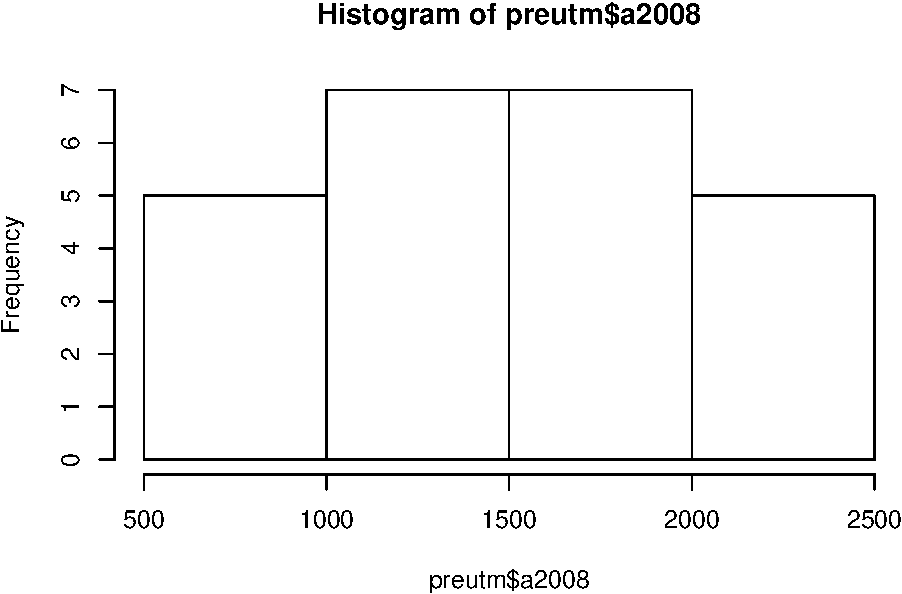
\includegraphics{proyecto_files/figure-latex/unnamed-chunk-25-1.pdf} *
Según el histograma normal, los datos presentan una distribución normal.

\subsubsection{Histogramas Logaritmica}\label{histogramas-logaritmica-1}

\begin{Shaded}
\begin{Highlighting}[]
\KeywordTok{hist}\NormalTok{(}\KeywordTok{log}\NormalTok{(preutm}\OperatorTok{$}\NormalTok{a2008))}
\end{Highlighting}
\end{Shaded}

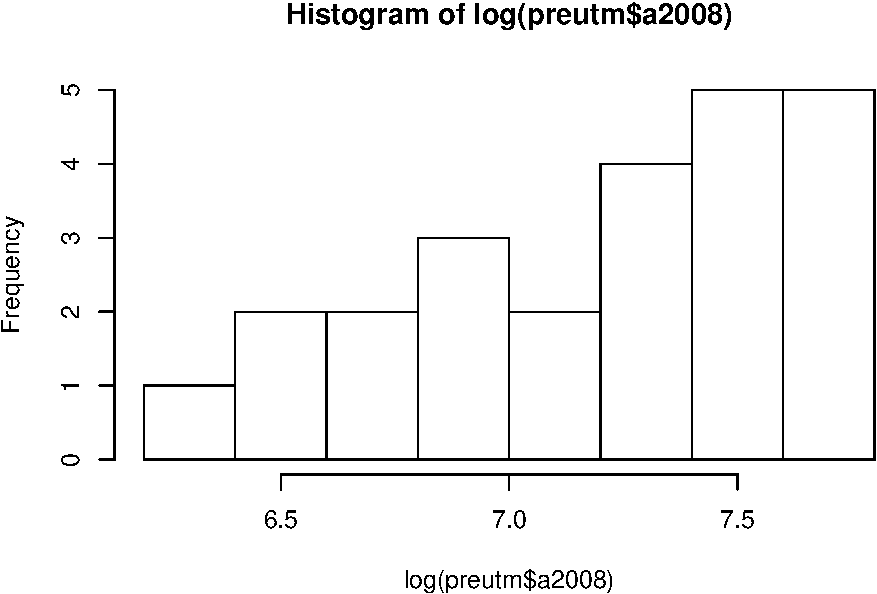
\includegraphics{proyecto_files/figure-latex/unnamed-chunk-26-1.pdf} *
Según este histograma logarítmico, los datos tienen una distribución
poco normal, porque para la derecha presenta la mayor cantidad de datos.

\subsection{Prueba de Shapiro-Wilk
Normal}\label{prueba-de-shapiro-wilk-normal-1}

\begin{Shaded}
\begin{Highlighting}[]
\KeywordTok{shapiro.test}\NormalTok{(preutm}\OperatorTok{$}\NormalTok{a2008)}
\end{Highlighting}
\end{Shaded}

\begin{verbatim}
## 
##  Shapiro-Wilk normality test
## 
## data:  preutm$a2008
## W = 0.9557, p-value = 0.3582
\end{verbatim}

\begin{itemize}
\tightlist
\item
  Según la prueba de Shapiro-Wilk Normal, el coeficiente significancia
  es mayor que 0.05 por tanto se acepta la hipótesis nula.
\end{itemize}

\subsubsection{Prueba de Shapiro-Wilk
Transformado}\label{prueba-de-shapiro-wilk-transformado-1}

\begin{Shaded}
\begin{Highlighting}[]
\KeywordTok{shapiro.test}\NormalTok{(}\KeywordTok{log}\NormalTok{(pre}\OperatorTok{$}\NormalTok{a2008))}
\end{Highlighting}
\end{Shaded}

\begin{verbatim}
## 
##  Shapiro-Wilk normality test
## 
## data:  log(pre$a2008)
## W = 0.93849, p-value = 0.1509
\end{verbatim}

\begin{itemize}
\tightlist
\item
  Según la prueba de Shapiro-Wilk, en la variable logarítmica el
  coeficiente de significancia es mayor que 0.05 por tanto se acepta la
  hipótesis nula, los datos vienen de una distribución normalmente
  distribuida.
\end{itemize}

\subsection{Precipitación del año
2008}\label{precipitaciuxf3n-del-auxf1o-2008}

\begin{Shaded}
\begin{Highlighting}[]
\NormalTok{pre2008 <-}\StringTok{ }\KeywordTok{na.omit}\NormalTok{(preutm[,}\KeywordTok{c}\NormalTok{(}\StringTok{'Estación', '}\NormalTok{a2008}\StringTok{')])}
\StringTok{pre2008}
\end{Highlighting}
\end{Shaded}

\begin{verbatim}
## Simple feature collection with 24 features and 2 fields
## geometry type:  POINT
## dimension:      XY
## bbox:           xmin: 215264.1 ymin: 1999092 xmax: 566794.7 ymax: 2197035
## epsg (SRID):    32619
## proj4string:    +proj=utm +zone=19 +datum=WGS84 +units=m +no_defs
## First 10 features:
##            Estación   a2008                     geom
## 1          Barahona 1136.80 POINT (277900.2 2013585)
## 2         Bayaguana 1831.20 POINT (433242.1 2073284)
## 4         Constanza 1072.90 POINT (320947.7 2090623)
## 5  Gaspar Hernández 1866.30 POINT (363678.2 2169619)
## 6       Hondo Valle 1399.15 POINT (215264.1 2071669)
## 7            Jimaní  751.10 POINT (221953.7 2045651)
## 8          La Unión 1536.30 POINT (337592.1 2184559)
## 9           La Vega 1072.90 POINT (338847.1 2125548)
## 10     Las Américas 1718.40 POINT (429562.7 2038222)
## 11             Moca 1144.30 POINT (342475.8 2143891)
\end{verbatim}

\subsection{Representacion de la Precipitación del año
2008}\label{representacion-de-la-precipitaciuxf3n-del-auxf1o-2008-1}

\begin{Shaded}
\begin{Highlighting}[]
\KeywordTok{library}\NormalTok{(ggplot2)}
\KeywordTok{ggplot}\NormalTok{() }\OperatorTok{+}
\StringTok{  }\KeywordTok{geom_sf}\NormalTok{(}\DataTypeTok{data =}\NormalTok{ prov, }\DataTypeTok{fill =} \StringTok{'white'}\NormalTok{) }\OperatorTok{+}
\StringTok{  }\KeywordTok{geom_sf}\NormalTok{(}\DataTypeTok{data =}\NormalTok{ pre2008, }\KeywordTok{aes}\NormalTok{(}\DataTypeTok{col =}\NormalTok{ a2008), }\DataTypeTok{size =} \DecValTok{6}\NormalTok{) }\OperatorTok{+}
\StringTok{  }\KeywordTok{scale_colour_gradient}\NormalTok{(}\DataTypeTok{low=}\StringTok{"#deebf7"}\NormalTok{, }\DataTypeTok{high=}\StringTok{"#3182bd"}\NormalTok{) }\OperatorTok{+}
\StringTok{  }\KeywordTok{geom_sf_text}\NormalTok{(}\DataTypeTok{data =}\NormalTok{ prov, }\KeywordTok{aes}\NormalTok{(}\DataTypeTok{label=}\NormalTok{TOPONIMIA), }\DataTypeTok{check_overlap =}\NormalTok{ T, }\DataTypeTok{size =} \DecValTok{2}\NormalTok{) }\OperatorTok{+}
\StringTok{  }\KeywordTok{geom_sf_text}\NormalTok{(}\DataTypeTok{data =}\NormalTok{ pre2008, }\KeywordTok{aes}\NormalTok{(}\DataTypeTok{label=}\NormalTok{Estación), }\DataTypeTok{check_overlap =}\NormalTok{ T, }\DataTypeTok{size =} \FloatTok{1.5}\NormalTok{) }\OperatorTok{+}
\StringTok{  }\KeywordTok{theme_bw}\NormalTok{()}
\end{Highlighting}
\end{Shaded}

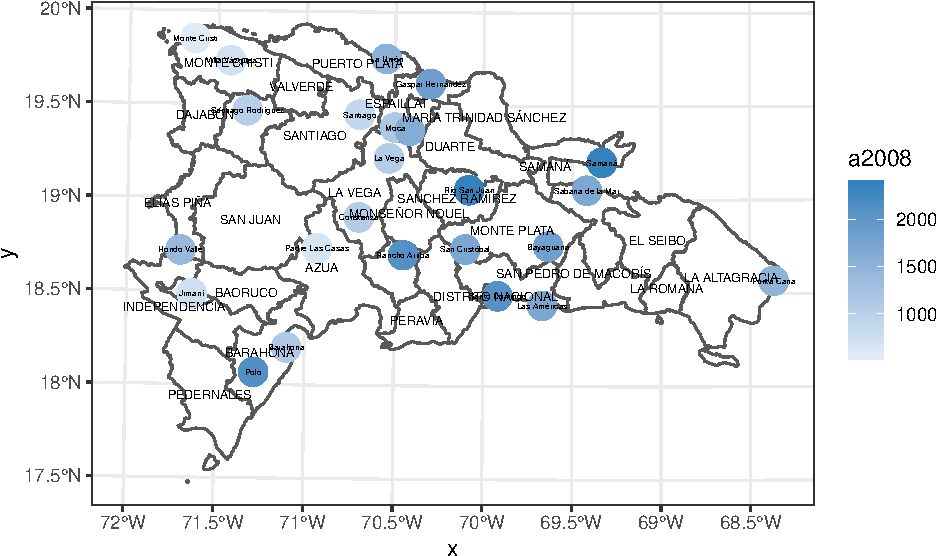
\includegraphics{proyecto_files/figure-latex/unnamed-chunk-30-1.pdf}

\begin{itemize}
\tightlist
\item
  Los valore de máximas precipitación están en los pluviómetros
  centrales y que tienen acceso a en los vientos alisios, las provincias
  como: Sánchez Ramírez, Monte Plata, María Trinidad Sánchez, Santo
  Domingo, Distrito Nacional San José de Ocoa, Hermanas Mirabal, San
  Cristóbal, Duarte, Semana, Barahona en (Polo) y Monseñor Noel. Donde
  hubo mediana precipitación es el Seíbo, Hato Mayor, La Romana, La
  Altagracia, Pedernales, Puerto Plata, Elia Piña, San Juan, Santiago y
  Santiago Rodríguez. En las demás provincias se evidencia baja
  precipitación.
\end{itemize}

\subsection{Variograma muestral}\label{variograma-muestral-1}

\begin{itemize}
\tightlist
\item
  Se Genera el variograma muestral para el logaritmo de la
  precipitación. Para esto se emplea la función variogram
\end{itemize}

\begin{Shaded}
\begin{Highlighting}[]
\NormalTok{v2008 <-}\StringTok{ }\KeywordTok{variogram}\NormalTok{(a2008}\OperatorTok{~}\DecValTok{1}\NormalTok{, pre2008)}
\NormalTok{v2008}
\end{Highlighting}
\end{Shaded}

\begin{verbatim}
##    np       dist     gamma dir.hor dir.ver   id
## 1   1   8896.559 109231.38       0       0 var1
## 2   7  22355.182 160973.45       0       0 var1
## 3  12  31950.749 140693.52       0       0 var1
## 4   7  40140.925  60776.08       0       0 var1
## 5   7  50078.452 444856.24       0       0 var1
## 6  13  58634.264 227820.90       0       0 var1
## 7   9  67157.152 202536.59       0       0 var1
## 8   8  77324.589 215532.06       0       0 var1
## 9  20  85454.491 238217.12       0       0 var1
## 10 12  93304.363 320335.94       0       0 var1
## 11  9 103937.517 129201.49       0       0 var1
## 12 19 112257.676 244612.55       0       0 var1
## 13 16 120305.537 269842.33       0       0 var1
## 14 13 128732.483 307869.87       0       0 var1
\end{verbatim}

\begin{Shaded}
\begin{Highlighting}[]
\KeywordTok{plot}\NormalTok{(v2008, }\DataTypeTok{plot.numbers =}\NormalTok{ T)}
\end{Highlighting}
\end{Shaded}

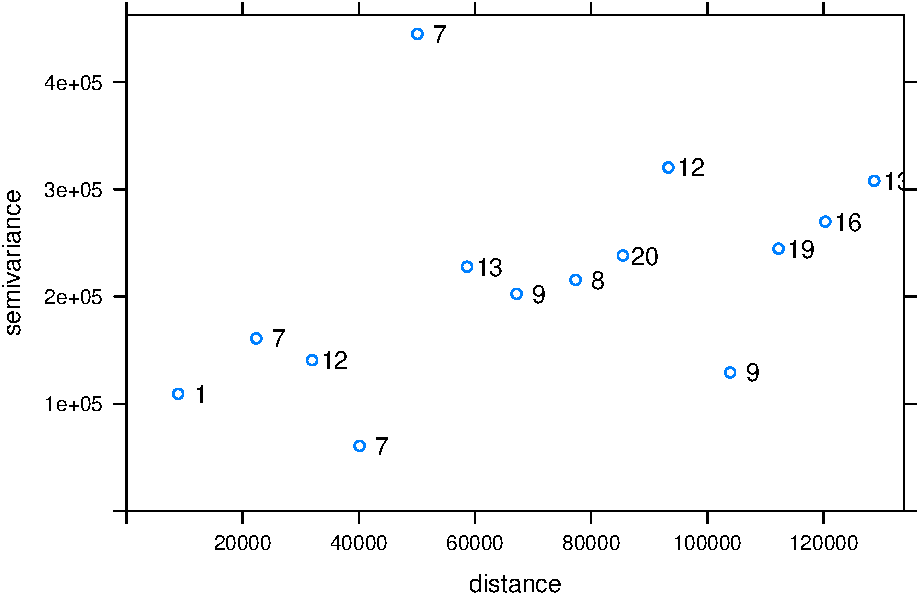
\includegraphics{proyecto_files/figure-latex/unnamed-chunk-31-1.pdf}

\subsubsection{Variograma Esferico}\label{variograma-esferico}

\begin{itemize}
\tightlist
\item
  Con el variograma muestral, se genera un variograma modelo que será el
  que se utlizará en la función krige para realizar la interpolación.
\end{itemize}

\begin{Shaded}
\begin{Highlighting}[]
\NormalTok{v2008_m <-}\StringTok{ }\KeywordTok{fit.variogram}\NormalTok{(v2008, }\KeywordTok{vgm}\NormalTok{(}\DataTypeTok{model =} \StringTok{"Sph"}\NormalTok{, }\DataTypeTok{range =} \DecValTok{50000}\NormalTok{))}
\NormalTok{v2008_m}
\end{Highlighting}
\end{Shaded}

\begin{verbatim}
##   model    psill    range
## 1   Sph 244665.2 60617.39
\end{verbatim}

\begin{Shaded}
\begin{Highlighting}[]
\KeywordTok{plot}\NormalTok{(v2008, v2008_m, }\DataTypeTok{plot.numbers =}\NormalTok{ T)}
\end{Highlighting}
\end{Shaded}

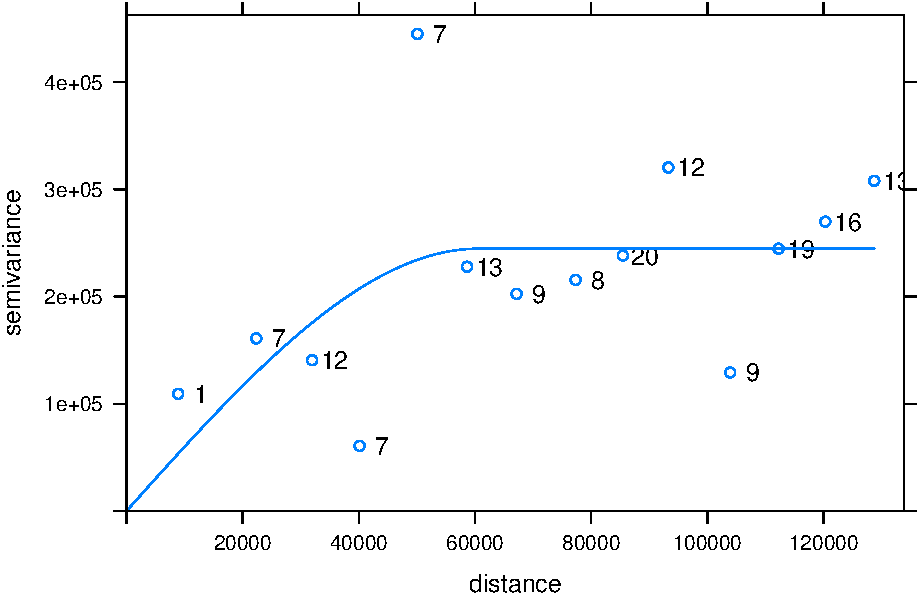
\includegraphics{proyecto_files/figure-latex/unnamed-chunk-32-1.pdf}

\subsubsection{Variograma modelo 2
(Exponencial)}\label{variograma-modelo-2-exponencial-1}

\begin{Shaded}
\begin{Highlighting}[]
\NormalTok{v2008_m2 <-}\StringTok{ }\KeywordTok{fit.variogram}\NormalTok{(v2008, }\KeywordTok{vgm}\NormalTok{(}\DataTypeTok{model =} \StringTok{"Exp"}\NormalTok{, }\DataTypeTok{range =} \DecValTok{50000}\NormalTok{))}
\NormalTok{v2008_m2}
\end{Highlighting}
\end{Shaded}

\begin{verbatim}
##   model    psill    range
## 1   Exp 250584.5 25586.33
\end{verbatim}

\begin{Shaded}
\begin{Highlighting}[]
\KeywordTok{plot}\NormalTok{(v2008, v2008_m2, }\DataTypeTok{plot.numbers =}\NormalTok{ T)}
\end{Highlighting}
\end{Shaded}

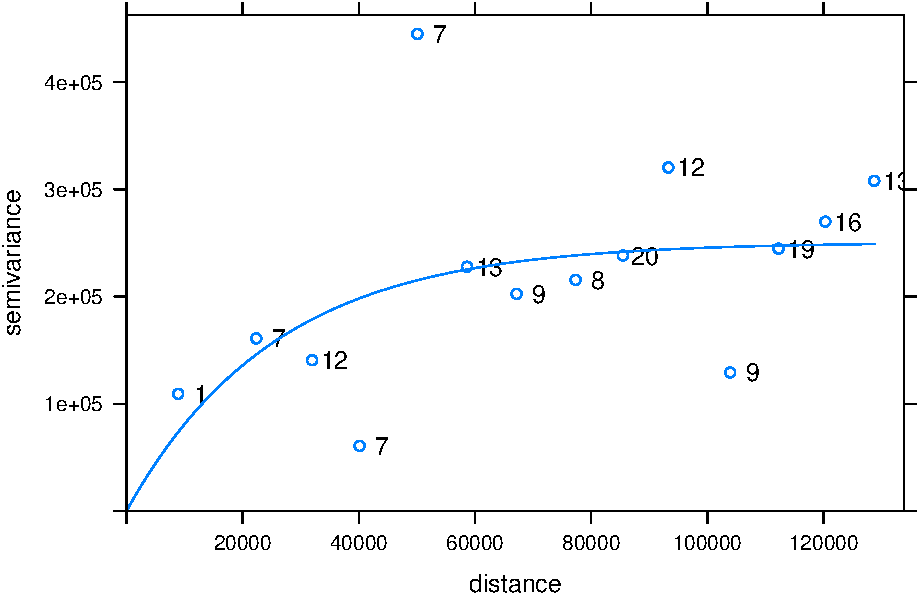
\includegraphics{proyecto_files/figure-latex/unnamed-chunk-33-1.pdf}

\subsubsection{Variograma modelo 3
(Gaussiano)}\label{variograma-modelo-3-gaussiano}

\begin{Shaded}
\begin{Highlighting}[]
\NormalTok{v2008_m3 <-}\StringTok{ }\KeywordTok{fit.variogram}\NormalTok{(v2008, }\KeywordTok{vgm}\NormalTok{(}\DataTypeTok{model =} \StringTok{"Gau"}\NormalTok{, }\DataTypeTok{range =} \DecValTok{50000}\NormalTok{))}
\NormalTok{v2008_m3}
\end{Highlighting}
\end{Shaded}

\begin{verbatim}
##   model    psill   range
## 1   Gau 188116.5 9599.91
\end{verbatim}

\begin{Shaded}
\begin{Highlighting}[]
\KeywordTok{plot}\NormalTok{(v2008, v2008_m3, }\DataTypeTok{plot.numbers =}\NormalTok{ T)}
\end{Highlighting}
\end{Shaded}

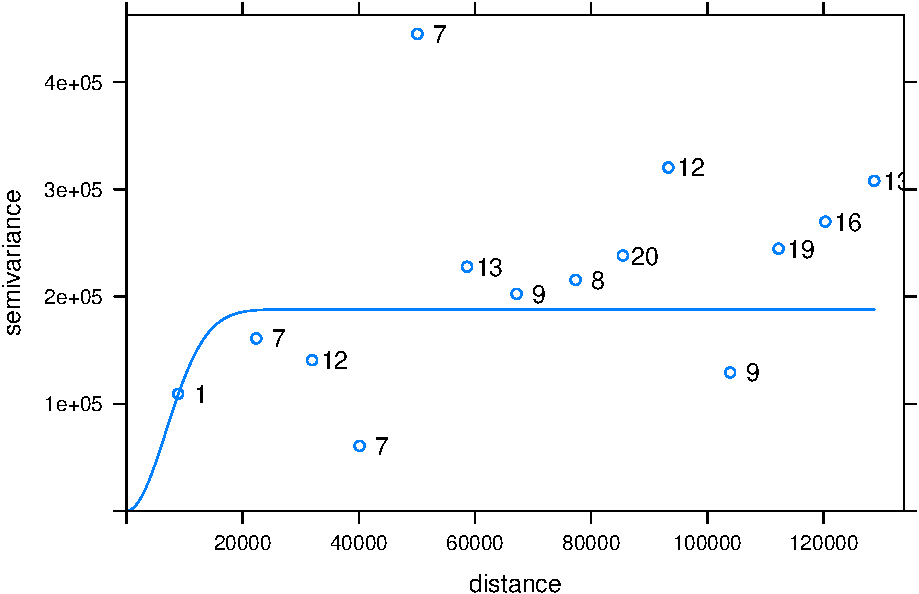
\includegraphics{proyecto_files/figure-latex/unnamed-chunk-34-1.pdf}

\begin{itemize}
\tightlist
\item
  De acuerdo a la representación gráfica de los diferentes Variogramas,
  el modelo que mejor se ajusta a los datos es el modelo Exponencial.
  Por lo que este será el usado para el procesado de los datos.
\end{itemize}

\subsection{Interpolación por Kriging
Ordinario}\label{interpolaciuxf3n-por-kriging-ordinario-1}

\begin{itemize}
\tightlist
\item
  Antes de realizar la interpolación, necesitamos una cuadrícula que
  ``llenaremos'' con las predicciones. Creamos una cuadrícula para RD,
  en este caso, de baja resolución, 10x10 km, esta cuadricula la vamos a
  crear con la libreria (stars)
\end{itemize}

\begin{Shaded}
\begin{Highlighting}[]
\NormalTok{grd <-}\StringTok{ }\KeywordTok{st_bbox}\NormalTok{(prov) }\OperatorTok
\StringTok{  }\KeywordTok{st_as_stars}\NormalTok{(}\DataTypeTok{dx =} \DecValTok{10000}\NormalTok{) }\OperatorTok\StringTok{ }\CommentTok{#10000 metros=1km de resolución espacial}
\StringTok{  }\KeywordTok{st_set_crs}\NormalTok{(crsdestino) }\OperatorTok
\StringTok{  }\KeywordTok{st_crop}\NormalTok{(prov)}
\NormalTok{grd}
\end{Highlighting}
\end{Shaded}

\begin{verbatim}
## stars object with 2 dimensions and 1 attribute
## attribute(s):
##     values    
##  Min.   :0    
##  1st Qu.:0    
##  Median :0    
##  Mean   :0    
##  3rd Qu.:0    
##  Max.   :0    
##  NA's   :605  
## dimension(s):
##   from to  offset  delta                       refsys point values    
## x    1 39  182216  10000 +proj=utm +zone=19 +datum...    NA   NULL [x]
## y    1 28 2205216 -10000 +proj=utm +zone=19 +datum...    NA   NULL [y]
\end{verbatim}

\begin{Shaded}
\begin{Highlighting}[]
\KeywordTok{plot}\NormalTok{(grd)}
\end{Highlighting}
\end{Shaded}

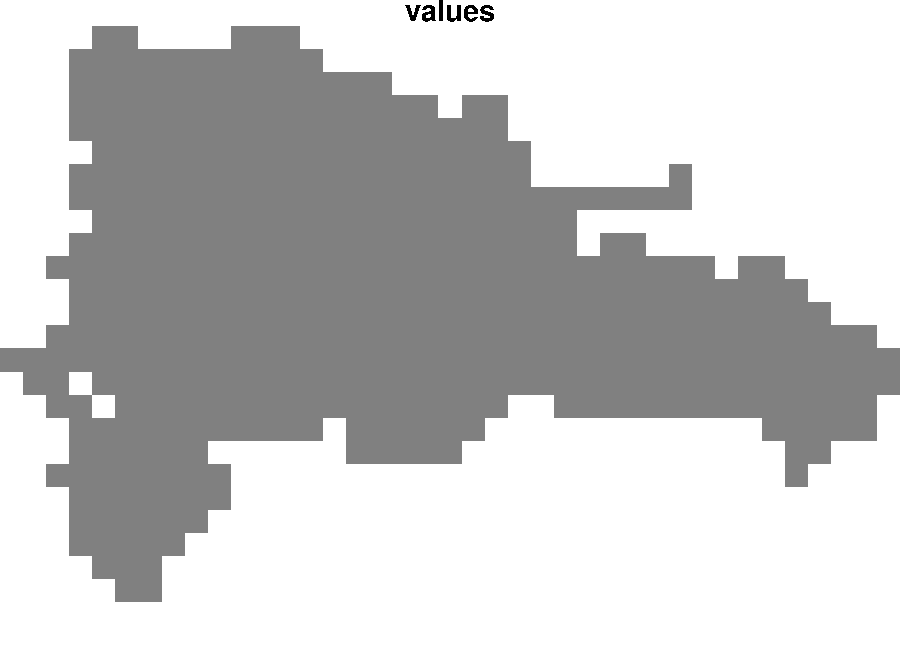
\includegraphics{proyecto_files/figure-latex/unnamed-chunk-35-1.pdf}

\subsubsection{Interpolacion Kriging}\label{interpolacion-kriging}

\begin{Shaded}
\begin{Highlighting}[]
\NormalTok{k <-}\StringTok{ }\KeywordTok{krige}\NormalTok{(}\DataTypeTok{formula =}\NormalTok{ a2008}\OperatorTok{~}\DecValTok{1}\NormalTok{, }\DataTypeTok{locations =}\NormalTok{ pre2008, }\DataTypeTok{newdata =}\NormalTok{ grd, }\DataTypeTok{model =}\NormalTok{ v2008_m2)}
\end{Highlighting}
\end{Shaded}

\begin{verbatim}
## [using ordinary kriging]
\end{verbatim}

\begin{Shaded}
\begin{Highlighting}[]
\NormalTok{k}
\end{Highlighting}
\end{Shaded}

\begin{verbatim}
## stars object with 2 dimensions and 2 attributes
## attribute(s):
##    var1.pred        var1.var      
##  Min.   : 671.6   Min.   : 29359  
##  1st Qu.:1181.6   1st Qu.:152996  
##  Median :1481.1   Median :200561  
##  Mean   :1445.4   Mean   :188528  
##  3rd Qu.:1703.2   3rd Qu.:230251  
##  Max.   :2264.0   Max.   :263269  
##  NA's   :605      NA's   :605     
## dimension(s):
##   from to  offset  delta                       refsys point values    
## x    1 39  182216  10000 +proj=utm +zone=19 +datum...    NA   NULL [x]
## y    1 28 2205216 -10000 +proj=utm +zone=19 +datum...    NA   NULL [y]
\end{verbatim}

\begin{Shaded}
\begin{Highlighting}[]
\KeywordTok{plot}\NormalTok{(k)}
\end{Highlighting}
\end{Shaded}

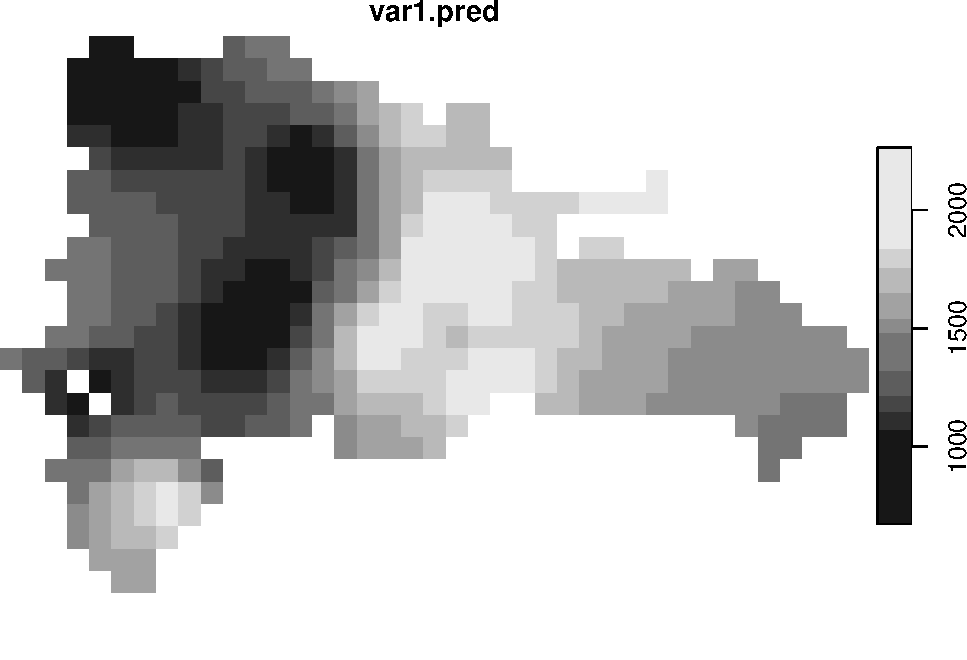
\includegraphics{proyecto_files/figure-latex/unnamed-chunk-36-1.pdf}

\subsubsection{Usar ggplot para representar el objeto
stars.}\label{usar-ggplot-para-representar-el-objeto-stars.-1}

\begin{Shaded}
\begin{Highlighting}[]
\KeywordTok{ggplot}\NormalTok{() }\OperatorTok{+}
\StringTok{  }\KeywordTok{geom_stars}\NormalTok{(}\DataTypeTok{data =}\NormalTok{ k, }\KeywordTok{aes}\NormalTok{(}\DataTypeTok{fill =}\NormalTok{ var1.pred, }\DataTypeTok{x =}\NormalTok{ x, }\DataTypeTok{y =}\NormalTok{ y)) }\OperatorTok{+}\StringTok{ }
\StringTok{  }\KeywordTok{scale_fill_gradient}\NormalTok{(}\DataTypeTok{low=}\StringTok{"#deebf7"}\NormalTok{, }\DataTypeTok{high=}\StringTok{"#3182bd"}\NormalTok{) }\OperatorTok{+}
\StringTok{  }\KeywordTok{geom_sf}\NormalTok{(}\DataTypeTok{data =} \KeywordTok{st_cast}\NormalTok{(prov, }\StringTok{"MULTILINESTRING"}\NormalTok{)) }\OperatorTok{+}
\StringTok{  }\KeywordTok{geom_sf}\NormalTok{(}\DataTypeTok{data =}\NormalTok{ pre2008) }\OperatorTok{+}
\StringTok{  }\KeywordTok{geom_sf_text}\NormalTok{(}\DataTypeTok{data =}\NormalTok{ prov, }\KeywordTok{aes}\NormalTok{(}\DataTypeTok{label=}\NormalTok{TOPONIMIA), }\DataTypeTok{check_overlap =}\NormalTok{ T, }\DataTypeTok{size =} \DecValTok{2}\NormalTok{, }\DataTypeTok{nudge_=}\DecValTok{500}\NormalTok{) }\OperatorTok{+}
\StringTok{  }\KeywordTok{theme_bw}\NormalTok{()}
\end{Highlighting}
\end{Shaded}

\begin{verbatim}
## Warning: Ignoring unknown parameters: nudge_
\end{verbatim}

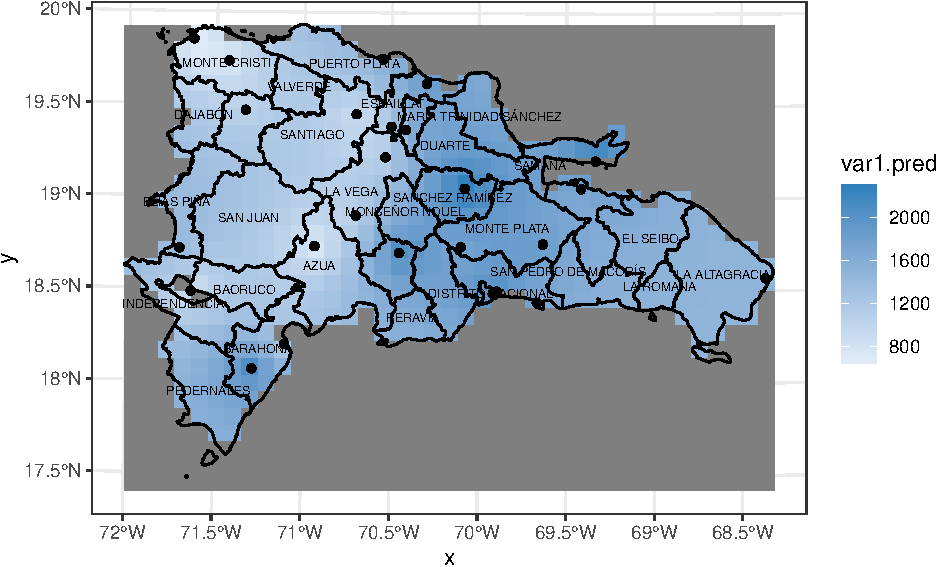
\includegraphics{proyecto_files/figure-latex/unnamed-chunk-37-1.pdf}

\begin{itemize}
\tightlist
\item
  Según el mapa, las provincias donde se evidencian que hubo mayores
  Precipitaciones son: Sánchez Ramírez, Monte Plata, María Trinidad
  Sánchez, Santo Domingo, Distrito Nacional San José de Ocoa, Hermanas
  Mirabal, San Cristóbal, Duarte, Semana, Barahona y Monseñor Noel.
  Donde hubo mediana precipitación es el Seíbo, Hato Mayor, La Romana,
  La Altagracia, Pedernales, Puerto Plata, Elia Piña, San Juan, Santiago
  y Santiago Rodríguez. En las demás provincias se evidencia baja
  precipitación.
\end{itemize}

\section*{Referencias}\label{referencias}
\addcontentsline{toc}{section}{Referencias}

\hypertarget{refs}{}
\hypertarget{ref-bivand2008applied}{}
Bivand, R. S., Pebesma, E. J., Gomez-Rubio, V., \& Pebesma, E. J.
(2008). \emph{Applied spatial data analysis with r} (Vol. 747248717).
Springer.

\hypertarget{ref-hengl2009practical}{}
Hengl, T. (2009). \emph{A practical guide to geostatistical mapping}
(Vol. 52). Hengl Amsterdam.

\hypertarget{ref-onamet2008precipitacion}{}
ONAMET. (2008). \emph{Precipitacion}. ONAMET.

\hypertarget{ref-one2012censo}{}
ONE. (2012). \emph{Censo}. ONE.

\hypertarget{ref-urenaevaluacion}{}
Ureña, F. I. C., \& Martínez, M. (n.d.). \emph{Evaluación de la
cobertura del ix censo nacional de población y vivienda 2010}.




\newpage
\singlespacing 
\end{document}
